% Options for packages loaded elsewhere
\PassOptionsToPackage{unicode}{hyperref}
\PassOptionsToPackage{hyphens}{url}
%
\documentclass[
]{book}
\usepackage{amsmath,amssymb}
\usepackage{lmodern}
\usepackage{iftex}
\ifPDFTeX
  \usepackage[T1]{fontenc}
  \usepackage[utf8]{inputenc}
  \usepackage{textcomp} % provide euro and other symbols
\else % if luatex or xetex
  \usepackage{unicode-math}
  \defaultfontfeatures{Scale=MatchLowercase}
  \defaultfontfeatures[\rmfamily]{Ligatures=TeX,Scale=1}
\fi
% Use upquote if available, for straight quotes in verbatim environments
\IfFileExists{upquote.sty}{\usepackage{upquote}}{}
\IfFileExists{microtype.sty}{% use microtype if available
  \usepackage[]{microtype}
  \UseMicrotypeSet[protrusion]{basicmath} % disable protrusion for tt fonts
}{}
\makeatletter
\@ifundefined{KOMAClassName}{% if non-KOMA class
  \IfFileExists{parskip.sty}{%
    \usepackage{parskip}
  }{% else
    \setlength{\parindent}{0pt}
    \setlength{\parskip}{6pt plus 2pt minus 1pt}}
}{% if KOMA class
  \KOMAoptions{parskip=half}}
\makeatother
\usepackage{xcolor}
\usepackage{color}
\usepackage{fancyvrb}
\newcommand{\VerbBar}{|}
\newcommand{\VERB}{\Verb[commandchars=\\\{\}]}
\DefineVerbatimEnvironment{Highlighting}{Verbatim}{commandchars=\\\{\}}
% Add ',fontsize=\small' for more characters per line
\usepackage{framed}
\definecolor{shadecolor}{RGB}{248,248,248}
\newenvironment{Shaded}{\begin{snugshade}}{\end{snugshade}}
\newcommand{\AlertTok}[1]{\textcolor[rgb]{0.94,0.16,0.16}{#1}}
\newcommand{\AnnotationTok}[1]{\textcolor[rgb]{0.56,0.35,0.01}{\textbf{\textit{#1}}}}
\newcommand{\AttributeTok}[1]{\textcolor[rgb]{0.77,0.63,0.00}{#1}}
\newcommand{\BaseNTok}[1]{\textcolor[rgb]{0.00,0.00,0.81}{#1}}
\newcommand{\BuiltInTok}[1]{#1}
\newcommand{\CharTok}[1]{\textcolor[rgb]{0.31,0.60,0.02}{#1}}
\newcommand{\CommentTok}[1]{\textcolor[rgb]{0.56,0.35,0.01}{\textit{#1}}}
\newcommand{\CommentVarTok}[1]{\textcolor[rgb]{0.56,0.35,0.01}{\textbf{\textit{#1}}}}
\newcommand{\ConstantTok}[1]{\textcolor[rgb]{0.00,0.00,0.00}{#1}}
\newcommand{\ControlFlowTok}[1]{\textcolor[rgb]{0.13,0.29,0.53}{\textbf{#1}}}
\newcommand{\DataTypeTok}[1]{\textcolor[rgb]{0.13,0.29,0.53}{#1}}
\newcommand{\DecValTok}[1]{\textcolor[rgb]{0.00,0.00,0.81}{#1}}
\newcommand{\DocumentationTok}[1]{\textcolor[rgb]{0.56,0.35,0.01}{\textbf{\textit{#1}}}}
\newcommand{\ErrorTok}[1]{\textcolor[rgb]{0.64,0.00,0.00}{\textbf{#1}}}
\newcommand{\ExtensionTok}[1]{#1}
\newcommand{\FloatTok}[1]{\textcolor[rgb]{0.00,0.00,0.81}{#1}}
\newcommand{\FunctionTok}[1]{\textcolor[rgb]{0.00,0.00,0.00}{#1}}
\newcommand{\ImportTok}[1]{#1}
\newcommand{\InformationTok}[1]{\textcolor[rgb]{0.56,0.35,0.01}{\textbf{\textit{#1}}}}
\newcommand{\KeywordTok}[1]{\textcolor[rgb]{0.13,0.29,0.53}{\textbf{#1}}}
\newcommand{\NormalTok}[1]{#1}
\newcommand{\OperatorTok}[1]{\textcolor[rgb]{0.81,0.36,0.00}{\textbf{#1}}}
\newcommand{\OtherTok}[1]{\textcolor[rgb]{0.56,0.35,0.01}{#1}}
\newcommand{\PreprocessorTok}[1]{\textcolor[rgb]{0.56,0.35,0.01}{\textit{#1}}}
\newcommand{\RegionMarkerTok}[1]{#1}
\newcommand{\SpecialCharTok}[1]{\textcolor[rgb]{0.00,0.00,0.00}{#1}}
\newcommand{\SpecialStringTok}[1]{\textcolor[rgb]{0.31,0.60,0.02}{#1}}
\newcommand{\StringTok}[1]{\textcolor[rgb]{0.31,0.60,0.02}{#1}}
\newcommand{\VariableTok}[1]{\textcolor[rgb]{0.00,0.00,0.00}{#1}}
\newcommand{\VerbatimStringTok}[1]{\textcolor[rgb]{0.31,0.60,0.02}{#1}}
\newcommand{\WarningTok}[1]{\textcolor[rgb]{0.56,0.35,0.01}{\textbf{\textit{#1}}}}
\usepackage{longtable,booktabs,array}
\usepackage{calc} % for calculating minipage widths
% Correct order of tables after \paragraph or \subparagraph
\usepackage{etoolbox}
\makeatletter
\patchcmd\longtable{\par}{\if@noskipsec\mbox{}\fi\par}{}{}
\makeatother
% Allow footnotes in longtable head/foot
\IfFileExists{footnotehyper.sty}{\usepackage{footnotehyper}}{\usepackage{footnote}}
\makesavenoteenv{longtable}
\usepackage{graphicx}
\makeatletter
\def\maxwidth{\ifdim\Gin@nat@width>\linewidth\linewidth\else\Gin@nat@width\fi}
\def\maxheight{\ifdim\Gin@nat@height>\textheight\textheight\else\Gin@nat@height\fi}
\makeatother
% Scale images if necessary, so that they will not overflow the page
% margins by default, and it is still possible to overwrite the defaults
% using explicit options in \includegraphics[width, height, ...]{}
\setkeys{Gin}{width=\maxwidth,height=\maxheight,keepaspectratio}
% Set default figure placement to htbp
\makeatletter
\def\fps@figure{htbp}
\makeatother
\setlength{\emergencystretch}{3em} % prevent overfull lines
\providecommand{\tightlist}{%
  \setlength{\itemsep}{0pt}\setlength{\parskip}{0pt}}
\setcounter{secnumdepth}{5}
\usepackage{booktabs}
\usepackage{booktabs}
\usepackage{longtable}
\usepackage{array}
\usepackage{multirow}
\usepackage{wrapfig}
\usepackage{float}
\usepackage{colortbl}
\usepackage{pdflscape}
\usepackage{tabu}
\usepackage{threeparttable}
\usepackage{threeparttablex}
\usepackage[normalem]{ulem}
\usepackage{makecell}
\usepackage{xcolor}
\ifLuaTeX
  \usepackage{selnolig}  % disable illegal ligatures
\fi
\usepackage[]{natbib}
\bibliographystyle{plainnat}
\IfFileExists{bookmark.sty}{\usepackage{bookmark}}{\usepackage{hyperref}}
\IfFileExists{xurl.sty}{\usepackage{xurl}}{} % add URL line breaks if available
\urlstyle{same} % disable monospaced font for URLs
\hypersetup{
  pdftitle={Supplementary Appendix for Beyond the Wire: US Military Deployments and Host Country Public Opinion},
  pdfauthor={Michael. A. Allen, Michael E. Flynn, Carla Martinez Machain, and Andrew Stravers},
  hidelinks,
  pdfcreator={LaTeX via pandoc}}

\title{Supplementary Appendix for Beyond the Wire: US Military Deployments and Host Country Public Opinion}
\author{Michael. A. Allen, Michael E. Flynn, Carla Martinez Machain, and Andrew Stravers}
\date{2022-10-11}

\usepackage{amsthm}
\newtheorem{theorem}{Theorem}[chapter]
\newtheorem{lemma}{Lemma}[chapter]
\newtheorem{corollary}{Corollary}[chapter]
\newtheorem{proposition}{Proposition}[chapter]
\newtheorem{conjecture}{Conjecture}[chapter]
\theoremstyle{definition}
\newtheorem{definition}{Definition}[chapter]
\theoremstyle{definition}
\newtheorem{example}{Example}[chapter]
\theoremstyle{definition}
\newtheorem{exercise}{Exercise}[chapter]
\theoremstyle{definition}
\newtheorem{hypothesis}{Hypothesis}[chapter]
\theoremstyle{remark}
\newtheorem*{remark}{Remark}
\newtheorem*{solution}{Solution}
\begin{document}
\maketitle

{
\setcounter{tocdepth}{1}
\tableofcontents
}
\hypertarget{summary}{%
\chapter*{Summary}\label{summary}}
\addcontentsline{toc}{chapter}{Summary}

This bookdown project contains additional supplementary information for the contents of our book, Beyond the Wire: US Military Deployments and the Diplomacy of Defense. The materials contained within include additional information on surveys, tables for the models presented in the book, additional figures, code for figures and tables, etc.

In general, we try to annotate the code to help users understand the various decisions we made throughout. Given the length of the manuscript and the sheer volume of code a line-by-line annotation isn't currently possible, but we will will provide a generally summary of denser material and highlight particular lines at more critical points in the workflow.

Also note that we try to load the appropriate libraries at the beginning of each appendix chapter, but some of these may be redundant or unused in the final iteration of the chapter. In many cases we also call the library as a part of the function call to ensure reproducability and avoid errors resulting from mistakenly calling a function from a different package (e.g.~\texttt{\{plyr::summarize\}} rather than \texttt{\{dplyr::summarize\}}).

This supplementary appendix generally follows the layout of the book and is comprised of separate chapters that contain information from the corresponding book chapter, with the exception of the theory chapter, which is largely lacking any data or accompanying code. The general layout is as follows:

\begin{enumerate}
\def\labelenumi{\arabic{enumi}.}
\tightlist
\item
  Introduction
\item
  Domain of Consent
\item
  Deployments and Contact
\item
  Deployments and Crime
\item
  Deployments and Minority Populations
\item
  Deployments and Protests
\item
  Domain of Competitive Consent
\end{enumerate}

All remaining errors are our own.

\hypertarget{introduction}{%
\chapter{Introduction}\label{introduction}}

The first chapter of the book largely focuses on providing background information on the project and exposition for the substance of the book. There are two figures displaying the location of US military personnel at two points in time (2005 and 2020).

Note that the one thing I changed on this page is the base size for the font. In the book it's set to 30, but this is necessary to get the figures to render properly given the output size. Here I've set the base size to 12 to achieve a more appropriate scaling. This also seems to be sensitive to whether you're using a Mac or Windows, so just a heads-up that getting this to render properly may require some tweaks on your end depending on your operating system.

\begin{Shaded}
\begin{Highlighting}[]
\CommentTok{\# Load libraries for itnroductory chapter}
\FunctionTok{library}\NormalTok{(tidyverse)}
\FunctionTok{library}\NormalTok{(tidyr)}
\FunctionTok{library}\NormalTok{(cshapes)}
\FunctionTok{library}\NormalTok{(maps)}
\FunctionTok{library}\NormalTok{(countrycode)}
\FunctionTok{library}\NormalTok{(scales)}
\FunctionTok{library}\NormalTok{(here)}
\FunctionTok{library}\NormalTok{(sf)}
\FunctionTok{library}\NormalTok{(rnaturalearth)}
\FunctionTok{library}\NormalTok{(rworldmap)}
\FunctionTok{library}\NormalTok{(viridis)}
\FunctionTok{library}\NormalTok{(sysfonts)}
\FunctionTok{library}\NormalTok{(showtext)}
\FunctionTok{library}\NormalTok{(knitr)}

\CommentTok{\# Set resolution to 400}
\NormalTok{knitr}\SpecialCharTok{::}\NormalTok{opts\_chunk}\SpecialCharTok{$}\FunctionTok{set}\NormalTok{(}\AttributeTok{comment =} \StringTok{\textquotesingle{}\textquotesingle{}}\NormalTok{, }\AttributeTok{dpi =} \DecValTok{400}\NormalTok{)}

\CommentTok{\# Use custom font from Google fonts}
\NormalTok{sysfonts}\SpecialCharTok{::}\FunctionTok{font\_add\_google}\NormalTok{(}\StringTok{"Oswald"}\NormalTok{, }\AttributeTok{family =} \StringTok{"oswald"}\NormalTok{)}
\NormalTok{showtext}\SpecialCharTok{::}\FunctionTok{showtext\_auto}\NormalTok{()}

\CommentTok{\# Set base font size for custom theme}
\NormalTok{basesize }\OtherTok{\textless{}{-}} \DecValTok{11} \CommentTok{\# Note this changed from book}

\CommentTok{\# Set custom theme}
\NormalTok{theme\_flynn\_map }\OtherTok{\textless{}{-}} \ControlFlowTok{function}\NormalTok{()\{}
  
  \FunctionTok{theme\_void}\NormalTok{(}\AttributeTok{base\_family =} \StringTok{"oswald"}\NormalTok{, }\AttributeTok{base\_size =}\NormalTok{ basesize) }\SpecialCharTok{\%+replace\%} 
    
    \FunctionTok{theme}\NormalTok{(}\AttributeTok{plot.title =} \FunctionTok{element\_text}\NormalTok{(}\AttributeTok{face =} \StringTok{"bold"}\NormalTok{, }\AttributeTok{size =}\NormalTok{ basesize, }\AttributeTok{hjust =} \DecValTok{0}\NormalTok{, }\AttributeTok{margin =} \FunctionTok{margin}\NormalTok{(}\AttributeTok{t =} \DecValTok{0}\NormalTok{, }\AttributeTok{b =} \FloatTok{0.3}\NormalTok{, }\AttributeTok{l =} \DecValTok{0}\NormalTok{, }\AttributeTok{r =} \DecValTok{0}\NormalTok{, }\AttributeTok{unit =} \StringTok{"cm"}\NormalTok{)),}
          \AttributeTok{plot.subtitle =} \FunctionTok{element\_text}\NormalTok{(}\AttributeTok{size =}\NormalTok{ basesize }\SpecialCharTok{*} \FloatTok{0.85}\NormalTok{, }\AttributeTok{hjust =} \DecValTok{0}\NormalTok{, }\AttributeTok{margin =} \FunctionTok{margin}\NormalTok{(}\AttributeTok{t =} \DecValTok{0}\NormalTok{, }\AttributeTok{b =} \FloatTok{0.3}\NormalTok{, }\AttributeTok{l =} \DecValTok{0}\NormalTok{, }\AttributeTok{r =} \DecValTok{0}\NormalTok{, }\AttributeTok{unit =} \StringTok{"cm"}\NormalTok{)),}
          \AttributeTok{plot.caption =} \FunctionTok{element\_text}\NormalTok{(}\AttributeTok{face =} \StringTok{"italic"}\NormalTok{, }\AttributeTok{size =}\NormalTok{ basesize }\SpecialCharTok{*} \FloatTok{0.65}\NormalTok{, }\AttributeTok{hjust =} \DecValTok{1}\NormalTok{, }\AttributeTok{margin =} \FunctionTok{margin}\NormalTok{(}\AttributeTok{t =} \FloatTok{0.2}\NormalTok{, }\AttributeTok{unit =} \StringTok{"cm"}\NormalTok{)),}
          \AttributeTok{plot.background =} \FunctionTok{element\_rect}\NormalTok{(}\AttributeTok{fill =} \StringTok{"white"}\NormalTok{, }\AttributeTok{color =} \StringTok{"white"}\NormalTok{),}
          \AttributeTok{strip.background =} \FunctionTok{element\_rect}\NormalTok{(}\AttributeTok{fill =} \StringTok{"gray80"}\NormalTok{, }\AttributeTok{color =} \StringTok{"black"}\NormalTok{),}
          \AttributeTok{strip.text =} \FunctionTok{element\_text}\NormalTok{(}\AttributeTok{color =} \StringTok{"black"}\NormalTok{, }\AttributeTok{face =} \StringTok{"bold"}\NormalTok{),}
          \AttributeTok{panel.grid.major =} \FunctionTok{element\_line}\NormalTok{(}\AttributeTok{color =} \StringTok{"white"}\NormalTok{, }\AttributeTok{size =} \DecValTok{0}\NormalTok{),}
          \AttributeTok{panel.grid.minor =} \FunctionTok{element\_line}\NormalTok{(}\AttributeTok{color =} \StringTok{"white"}\NormalTok{, }\AttributeTok{size =} \DecValTok{0}\NormalTok{),}
          \CommentTok{\#axis.title = element\_text(face = "bold", size = 0),}
          \CommentTok{\#axis.title.y = element\_text(margin = margin(t = 0, r = 0.5, b = 0, l = 0, unit = "cm")),}
          \CommentTok{\#axis.title.x = element\_text(margin = margin(t = 0.5, r = 0, b = 0, l = 0, unit = "cm")),}
          \AttributeTok{legend.title =} \FunctionTok{element\_text}\NormalTok{(}\AttributeTok{face =} \StringTok{"bold"}\NormalTok{, }\AttributeTok{lineheight =} \FloatTok{1.2}\NormalTok{),}
          \AttributeTok{legend.position =} \StringTok{"bottom"}\NormalTok{,}
          \AttributeTok{legend.key.height =} \FunctionTok{unit}\NormalTok{(}\FloatTok{0.6}\NormalTok{, }\StringTok{"cm"}\NormalTok{),}
          \AttributeTok{legend.key.width =} \FunctionTok{unit}\NormalTok{(}\FloatTok{2.5}\NormalTok{, }\StringTok{"cm"}\NormalTok{))}
\NormalTok{\}}


\CommentTok{\# Set Seed}
\NormalTok{SEED }\OtherTok{\textless{}{-}} \DecValTok{66502}
\FunctionTok{set.seed}\NormalTok{(}\AttributeTok{seed =}\NormalTok{ SEED)}
\end{Highlighting}
\end{Shaded}

\begin{Shaded}
\begin{Highlighting}[]
\CommentTok{\# Use the troopdata function to obtain deployment data for 1950.}
\NormalTok{troop.data }\OtherTok{\textless{}{-}}\NormalTok{ troopdata}\SpecialCharTok{::}\FunctionTok{get\_troopdata}\NormalTok{(}\AttributeTok{startyear =} \DecValTok{1950}\NormalTok{, }\AttributeTok{endyear =} \DecValTok{1950}\NormalTok{) }\SpecialCharTok{\%\textgreater{}\%} 
  \CommentTok{\# Remove US from data}
  \FunctionTok{filter}\NormalTok{(ccode }\SpecialCharTok{!=} \DecValTok{2}\NormalTok{) }\SpecialCharTok{\%\textgreater{}\%} 
  \CommentTok{\# Change West Germany\textquotesingle{}s code from 260 to 255}
  \FunctionTok{mutate}\NormalTok{(}\AttributeTok{ccode =} \FunctionTok{ifelse}\NormalTok{(ccode }\SpecialCharTok{==} \DecValTok{260}\NormalTok{, }\DecValTok{255}\NormalTok{, ccode))}
\end{Highlighting}
\end{Shaded}

\begin{verbatim}
Warning: Data include troop values for unknown locations and personnel listed as
'afloat'.
\end{verbatim}

\begin{Shaded}
\begin{Highlighting}[]
\CommentTok{\# Use naturalearth package to create basemap.}
\NormalTok{map.base }\OtherTok{\textless{}{-}}\NormalTok{ rnaturalearth}\SpecialCharTok{::}\FunctionTok{ne\_countries}\NormalTok{(}\AttributeTok{returnclass =} \StringTok{"sf"}\NormalTok{)}

\CommentTok{\# Use cshapes package to generate COW system data for 1950}
\NormalTok{map}\FloatTok{.1950} \OtherTok{\textless{}{-}} \FunctionTok{cshp}\NormalTok{(}\AttributeTok{date =} \FunctionTok{as.Date}\NormalTok{(}\StringTok{"1950{-}01{-}01"}\NormalTok{)) }\SpecialCharTok{\%\textgreater{}\%}  
\NormalTok{  dplyr}\SpecialCharTok{::}\FunctionTok{mutate}\NormalTok{(., }\AttributeTok{ccode =}\NormalTok{ countrycode}\SpecialCharTok{::}\FunctionTok{countrycode}\NormalTok{(gwcode, }\StringTok{"gwn"}\NormalTok{, }\StringTok{"cown"}\NormalTok{)) }\SpecialCharTok{\%\textgreater{}\%} 
  \FunctionTok{left\_join}\NormalTok{(troop.data, }\AttributeTok{by =} \StringTok{"ccode"}\NormalTok{)}
\end{Highlighting}
\end{Shaded}

\begin{verbatim}
Warning in countrycode_convert(sourcevar = sourcevar, origin = origin, destination = dest, : Some values were not matched unambiguously: 711
\end{verbatim}

\begin{Shaded}
\begin{Highlighting}[]
\CommentTok{\# Use ggplot and sf packages to create map of 1950 deployments}
\CommentTok{\# Lay down base map first then deployments}
\CommentTok{\# Note the application of the coordinate reference system below to alter projection from default}
\FunctionTok{ggplot}\NormalTok{() }\SpecialCharTok{+}
  \FunctionTok{geom\_sf}\NormalTok{(}\AttributeTok{data =}\NormalTok{ map.base, }\FunctionTok{aes}\NormalTok{(}\AttributeTok{geometry =}\NormalTok{ geometry), }\AttributeTok{fill =} \StringTok{"gray90"}\NormalTok{, }\AttributeTok{color =} \StringTok{"gray90"}\NormalTok{, }\AttributeTok{size =} \FloatTok{0.1}\NormalTok{) }\SpecialCharTok{+}
  \FunctionTok{geom\_sf}\NormalTok{(}\AttributeTok{data =}\NormalTok{ map}\FloatTok{.1950}\NormalTok{, }\FunctionTok{aes}\NormalTok{(}\AttributeTok{geometry =}\NormalTok{ geometry, }\AttributeTok{fill =}\NormalTok{ troops), }\AttributeTok{color =} \StringTok{"white"}\NormalTok{, }\AttributeTok{size =} \FloatTok{0.1}\NormalTok{) }\SpecialCharTok{+}
  \FunctionTok{theme\_flynn\_map}\NormalTok{() }\SpecialCharTok{+}
  \FunctionTok{theme}\NormalTok{(}\AttributeTok{legend.text =} \FunctionTok{element\_text}\NormalTok{(}\AttributeTok{size =}\NormalTok{ basesize}\SpecialCharTok{*}\FloatTok{1.05}\NormalTok{, }\AttributeTok{margin =} \FunctionTok{margin}\NormalTok{(}\AttributeTok{t =} \SpecialCharTok{{-}}\DecValTok{6}\NormalTok{, }\AttributeTok{unit =} \StringTok{"pt"}\NormalTok{)),}
        \AttributeTok{legend.title =} \FunctionTok{element\_text}\NormalTok{(}\AttributeTok{size =}\NormalTok{ basesize}\SpecialCharTok{*}\FloatTok{1.1}\NormalTok{, }\AttributeTok{lineheight =} \FloatTok{0.3}\NormalTok{),}
        \AttributeTok{plot.margin =} \FunctionTok{margin}\NormalTok{(}\DecValTok{0}\NormalTok{, }\DecValTok{0}\NormalTok{, }\DecValTok{0}\NormalTok{, }\DecValTok{0}\NormalTok{)) }\SpecialCharTok{+}
\NormalTok{  viridis}\SpecialCharTok{::}\FunctionTok{scale\_fill\_viridis}\NormalTok{(}\AttributeTok{option =} \StringTok{"magma"}\NormalTok{, }\AttributeTok{direction =} \SpecialCharTok{{-}}\DecValTok{1}\NormalTok{, }\AttributeTok{begin =} \FloatTok{0.1}\NormalTok{, }\AttributeTok{end =} \FloatTok{0.9}\NormalTok{, }\AttributeTok{na.value =} \StringTok{"gray90"}\NormalTok{, }\AttributeTok{breaks =} \FunctionTok{c}\NormalTok{(}\DecValTok{0}\NormalTok{, }\DecValTok{20}\NormalTok{, }\DecValTok{200}\NormalTok{, }\DecValTok{2000}\NormalTok{, }\DecValTok{20000}\NormalTok{, }\DecValTok{200000}\NormalTok{), }\AttributeTok{limits =} \FunctionTok{c}\NormalTok{(}\DecValTok{0}\NormalTok{, }\DecValTok{200000}\NormalTok{), }\AttributeTok{trans =} \StringTok{"log1p"}\NormalTok{, }\AttributeTok{label =} \FunctionTok{comma\_format}\NormalTok{()) }\SpecialCharTok{+}
  \FunctionTok{coord\_sf}\NormalTok{(}\AttributeTok{crs =} \FunctionTok{st\_crs}\NormalTok{(}\StringTok{"ESRI:54030"}\NormalTok{)) }\SpecialCharTok{+}
  \FunctionTok{labs}\NormalTok{(}\AttributeTok{fill =} \StringTok{"Deployment}\SpecialCharTok{\textbackslash{}n}\StringTok{Size"}\NormalTok{)}
\end{Highlighting}
\end{Shaded}

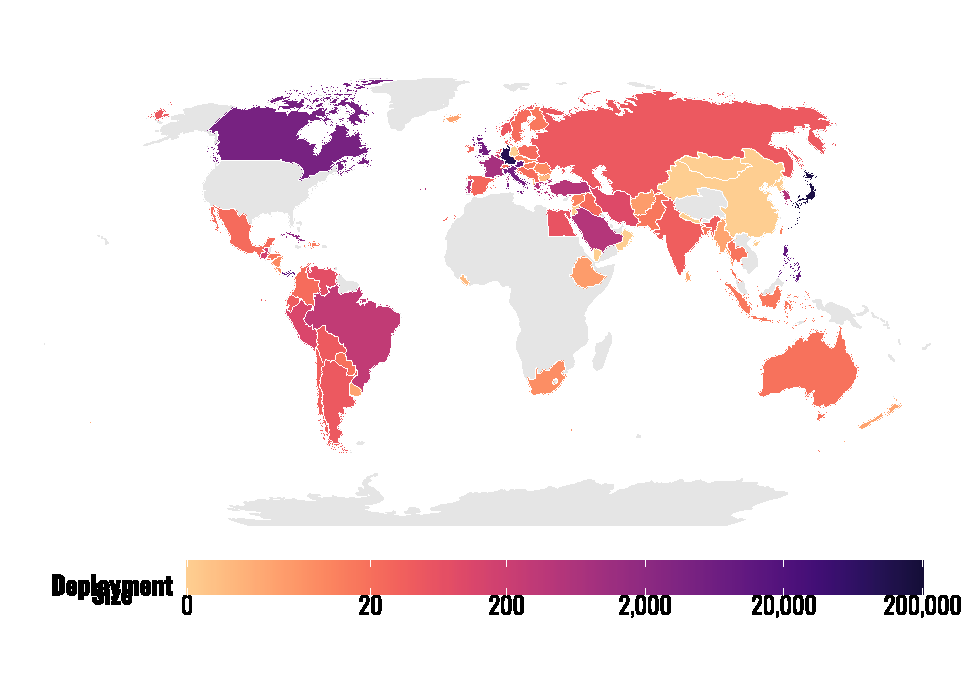
\includegraphics{01-introduction_files/figure-latex/maps of deployments in 1950-1.pdf}

\begin{Shaded}
\begin{Highlighting}[]
\CommentTok{\# As above, use troopdata package to get deployment data for 2020. Remove US, and change West Germany\textquotesingle{}s country code.}
\NormalTok{troop.data }\OtherTok{\textless{}{-}}\NormalTok{ troopdata}\SpecialCharTok{::}\FunctionTok{get\_troopdata}\NormalTok{(}\AttributeTok{startyear =} \DecValTok{2020}\NormalTok{, }\AttributeTok{endyear =} \DecValTok{2020}\NormalTok{) }\SpecialCharTok{\%\textgreater{}\%} 
  \FunctionTok{filter}\NormalTok{(ccode }\SpecialCharTok{!=} \DecValTok{2}\NormalTok{) }\SpecialCharTok{\%\textgreater{}\%} 
  \FunctionTok{mutate}\NormalTok{(}\AttributeTok{ccode =} \FunctionTok{ifelse}\NormalTok{(ccode }\SpecialCharTok{==} \DecValTok{260}\NormalTok{, }\DecValTok{255}\NormalTok{, ccode))}
\end{Highlighting}
\end{Shaded}

\begin{verbatim}
Warning: Data include troop values for unknown locations and personnel listed as
'afloat'.
\end{verbatim}

\begin{Shaded}
\begin{Highlighting}[]
\CommentTok{\# Use naturalearth package to create basemap.}
\NormalTok{map.base }\OtherTok{\textless{}{-}}\NormalTok{ rnaturalearth}\SpecialCharTok{::}\FunctionTok{ne\_countries}\NormalTok{(}\AttributeTok{returnclass =} \StringTok{"sf"}\NormalTok{)}

\NormalTok{map}\FloatTok{.2020} \OtherTok{\textless{}{-}}\NormalTok{ cshapes}\SpecialCharTok{::}\FunctionTok{cshp}\NormalTok{(}\AttributeTok{date =} \FunctionTok{as.Date}\NormalTok{(}\StringTok{"2019{-}01{-}01"}\NormalTok{)) }\SpecialCharTok{\%\textgreater{}\%}  
\NormalTok{  dplyr}\SpecialCharTok{::}\FunctionTok{mutate}\NormalTok{(., }\AttributeTok{ccode =}\NormalTok{ countrycode}\SpecialCharTok{::}\FunctionTok{countrycode}\NormalTok{(gwcode, }\StringTok{"gwn"}\NormalTok{, }\StringTok{"cown"}\NormalTok{)) }\SpecialCharTok{\%\textgreater{}\%} 
  \FunctionTok{left\_join}\NormalTok{(troop.data, }\AttributeTok{by =} \StringTok{"ccode"}\NormalTok{)}
\end{Highlighting}
\end{Shaded}

\begin{verbatim}
Warning in countrycode_convert(sourcevar = sourcevar, origin = origin, destination = dest, : Some values were not matched unambiguously: 340, 816
\end{verbatim}

\begin{Shaded}
\begin{Highlighting}[]
\CommentTok{\# Use ggplot and sf packages to create map of 1950 deployments}
\CommentTok{\# Lay down base map first then deployments}
\CommentTok{\# Note the application of the coordinate reference system below to alter projection from default}
\FunctionTok{ggplot}\NormalTok{() }\SpecialCharTok{+}
  \FunctionTok{geom\_sf}\NormalTok{(}\AttributeTok{data =}\NormalTok{ map.base, }\FunctionTok{aes}\NormalTok{(}\AttributeTok{geometry =}\NormalTok{ geometry), }\AttributeTok{fill =} \StringTok{"gray90"}\NormalTok{, }\AttributeTok{color =} \StringTok{"gray90"}\NormalTok{, }\AttributeTok{size =} \FloatTok{0.1}\NormalTok{) }\SpecialCharTok{+}
  \FunctionTok{geom\_sf}\NormalTok{(}\AttributeTok{data =}\NormalTok{ map}\FloatTok{.2020}\NormalTok{, }\FunctionTok{aes}\NormalTok{(}\AttributeTok{geometry =}\NormalTok{ geometry, }\AttributeTok{fill =}\NormalTok{ troops), }\AttributeTok{color =} \StringTok{"white"}\NormalTok{, }\AttributeTok{size =} \FloatTok{0.1}\NormalTok{) }\SpecialCharTok{+}
  \FunctionTok{theme\_flynn\_map}\NormalTok{() }\SpecialCharTok{+}
  \FunctionTok{theme}\NormalTok{(}\AttributeTok{legend.text =} \FunctionTok{element\_text}\NormalTok{(}\AttributeTok{size =}\NormalTok{ basesize}\SpecialCharTok{*}\FloatTok{1.05}\NormalTok{, }\AttributeTok{margin =} \FunctionTok{margin}\NormalTok{(}\AttributeTok{t =} \SpecialCharTok{{-}}\DecValTok{6}\NormalTok{, }\AttributeTok{unit =} \StringTok{"pt"}\NormalTok{)),}
        \AttributeTok{legend.title =} \FunctionTok{element\_text}\NormalTok{(}\AttributeTok{size =}\NormalTok{ basesize}\SpecialCharTok{*}\FloatTok{1.1}\NormalTok{, }\AttributeTok{lineheight =} \FloatTok{0.3}\NormalTok{),}
        \AttributeTok{plot.margin =} \FunctionTok{margin}\NormalTok{(}\DecValTok{0}\NormalTok{, }\DecValTok{0}\NormalTok{, }\DecValTok{0}\NormalTok{, }\DecValTok{0}\NormalTok{)) }\SpecialCharTok{+}
\NormalTok{  viridis}\SpecialCharTok{::}\FunctionTok{scale\_fill\_viridis}\NormalTok{(}\AttributeTok{option =} \StringTok{"magma"}\NormalTok{, }\AttributeTok{direction =} \SpecialCharTok{{-}}\DecValTok{1}\NormalTok{, }\AttributeTok{begin =} \FloatTok{0.1}\NormalTok{, }\AttributeTok{end =} \FloatTok{0.9}\NormalTok{, }\AttributeTok{na.value =} \StringTok{"gray90"}\NormalTok{, }\AttributeTok{breaks =} \FunctionTok{c}\NormalTok{(}\DecValTok{0}\NormalTok{, }\DecValTok{20}\NormalTok{, }\DecValTok{200}\NormalTok{, }\DecValTok{2000}\NormalTok{, }\DecValTok{20000}\NormalTok{, }\DecValTok{200000}\NormalTok{), }\AttributeTok{limits =} \FunctionTok{c}\NormalTok{(}\DecValTok{0}\NormalTok{, }\DecValTok{200000}\NormalTok{), }\AttributeTok{trans =} \StringTok{"log1p"}\NormalTok{, }\AttributeTok{label =} \FunctionTok{comma\_format}\NormalTok{()) }\SpecialCharTok{+}
  \FunctionTok{coord\_sf}\NormalTok{(}\AttributeTok{crs =} \FunctionTok{st\_crs}\NormalTok{(}\StringTok{"ESRI:54030"}\NormalTok{)) }\SpecialCharTok{+}
  \FunctionTok{labs}\NormalTok{(}\AttributeTok{fill =} \StringTok{"Deployment}\SpecialCharTok{\textbackslash{}n}\StringTok{Size"}\NormalTok{)}
\end{Highlighting}
\end{Shaded}

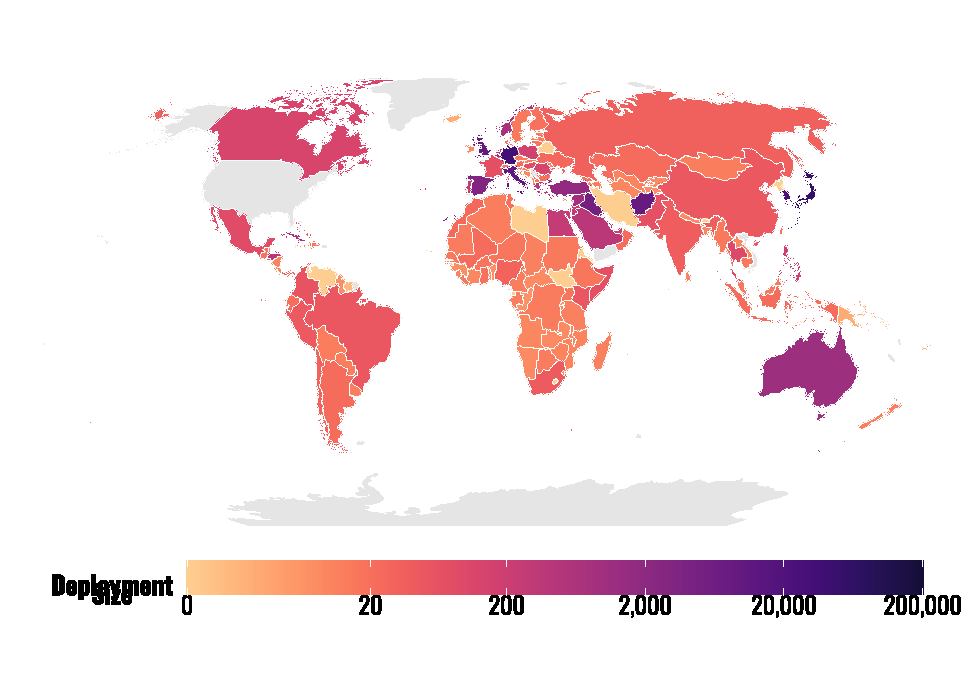
\includegraphics{01-introduction_files/figure-latex/maps of deployments in 2020-1.pdf}

\hypertarget{contact-benefits}{%
\chapter{Deployments and Contact}\label{contact-benefits}}

This chapter contains supplementary information on the chapter exploring how contact and benefits relate to individual attitudes.

\hypertarget{descriptive-information}{%
\section{Descriptive Information}\label{descriptive-information}}

\begin{figure}
\centering
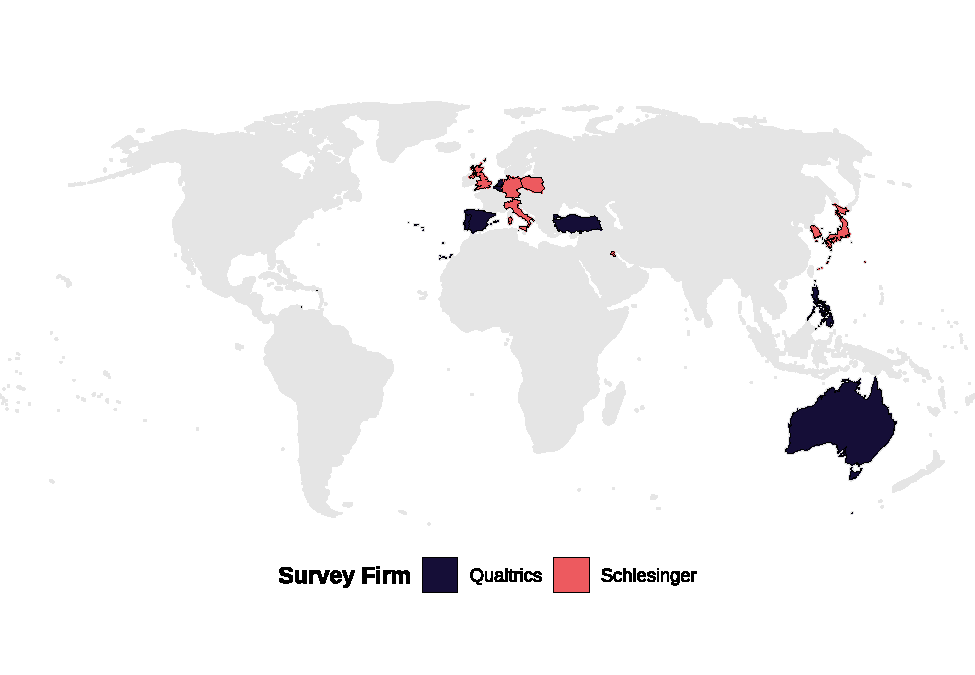
\includegraphics{02-contact-benefits_files/figure-latex/unnamed-chunk-1-1.pdf}
\caption{\label{fig:unnamed-chunk-1}Map of countries included in the survey. Color coding indicates which survey firm fielded the surveys in a given country.}
\end{figure}

Summary statistics detailing breakdown of views.

One detail that we wanted to convey in the book was just how out of step views of the US government often are compared with views of US military personnel and the American people. Figure \ref{fig:gov-gap} shows these differences by showing the percent of people in each country who responded with a favorable or unfavorable view of the group listed on the X axis.

\begin{figure}
\centering
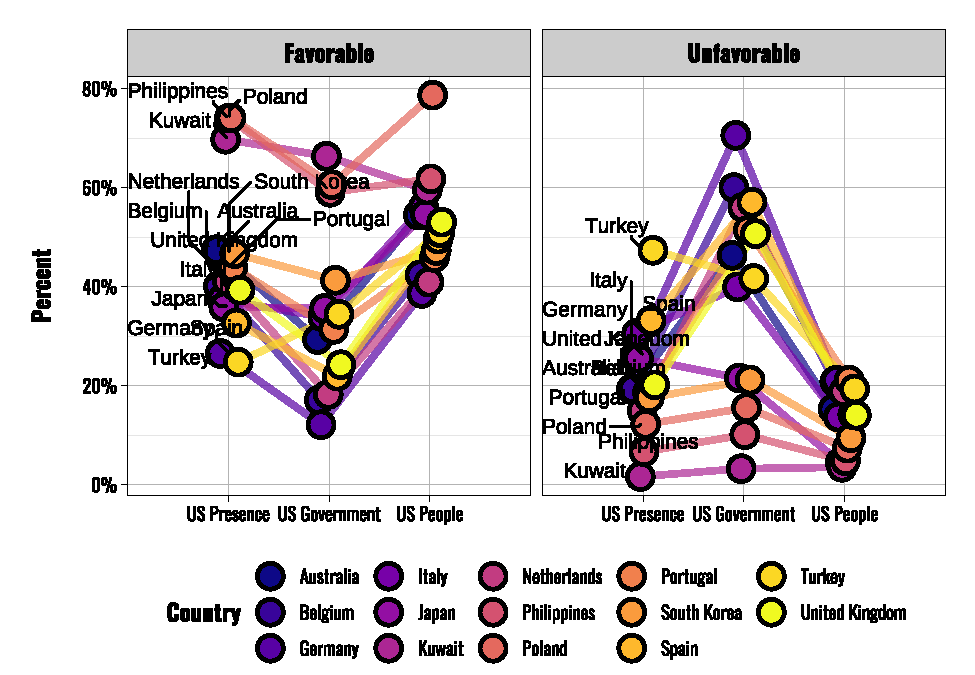
\includegraphics{02-contact-benefits_files/figure-latex/gov-gap-1.pdf}
\caption{\label{fig:gov-gap}Favorable and Unfavorable views of US actors. Categories aggregated to favorable and unfavorable based on a response of `Somewhat' or `Very'.}
\end{figure}

For more detail how the countries vary in terms of reported forms of contact and benefits, Table \ref{tab:contact-benefits-summary} shows the proportion of people responding ``Yes'' in each country when asked about their contact experience or whether they receive personal economic benefits from a US military presence, or if they know someone who receives such an economic benefit.

\begin{table}

\caption{\label{tab:contact-benefits-summary}Breakdown of the proportion of individuals who responded 'Yes' to key contact and benefit questions in each country.}
\centering
\fontsize{11}{13}\selectfont
\begin{tabular}[t]{l|r|r|r|r}
\hline
Country & Personal Contact & Personal Benefits & Network Contact & Network Benefits\\
\hline
Australia & 0.106 & 0.049 & 0.109 & 0.049\\
\hline
Belgium & 0.100 & 0.060 & 0.118 & 0.068\\
\hline
Germany & 0.251 & 0.049 & 0.246 & 0.072\\
\hline
Italy & 0.092 & 0.046 & 0.115 & 0.067\\
\hline
Japan & 0.084 & 0.033 & 0.080 & 0.033\\
\hline
Kuwait & 0.328 & 0.337 & 0.345 & 0.345\\
\hline
Netherlands & 0.084 & 0.062 & 0.093 & 0.076\\
\hline
Philippines & 0.143 & 0.154 & 0.192 & 0.217\\
\hline
Poland & 0.118 & 0.094 & 0.156 & 0.082\\
\hline
Portugal & 0.096 & 0.052 & 0.127 & 0.063\\
\hline
South Korea & 0.159 & 0.046 & 0.175 & 0.079\\
\hline
Spain & 0.096 & 0.040 & 0.102 & 0.060\\
\hline
Turkey & 0.117 & 0.113 & 0.128 & 0.126\\
\hline
United Kingdom & 0.137 & 0.071 & 0.143 & 0.080\\
\hline
\end{tabular}
\end{table}

\hypertarget{supplemental-information-on-models}{%
\section{Supplemental Information on Models}\label{supplemental-information-on-models}}

\hypertarget{prior-specification-tables}{%
\subsection{Prior Specification Tables}\label{prior-specification-tables}}

\begin{table}

\caption{\label{tab:prior-info-troops}Priors specifications for Troops contact models.}
\centering
\fontsize{11}{13}\selectfont
\begin{tabular}[t]{l|l|l|l|l|l|l|l|l|l}
\hline
prior & class & coef & group & resp & dpar & nlpar & lb & ub & source\\
\hline
normal(0,3) & Intercept &  &  &  & mudk &  &  &  & default\\
\hline
normal(0,3) & Intercept &  &  &  & muneg &  &  &  & default\\
\hline
normal(0,3) & Intercept &  &  &  & mupos &  &  &  & default\\
\hline
lkj\_corr\_cholesky(1) & L &  &  &  &  &  &  &  & default\\
\hline
 & L &  & country &  &  &  &  &  & default\\
\hline
normal(0,2) & b &  &  &  & mudk &  &  &  & default\\
\hline
normal(-0.16,0.17) & b & age25to34years &  &  & mudk &  &  &  & \\
\hline
normal(-0.41,0.17) & b & age35to44years &  &  & mudk &  &  &  & \\
\hline
normal(-0.36,0.18) & b & age45to54years &  &  & mudk &  &  &  & \\
\hline
normal(-0.75,0.19) & b & age55to64years &  &  & mudk &  &  &  & \\
\hline
normal(-0.98,0.23) & b & ageAge65orolder &  &  & mudk &  &  &  & \\
\hline
normal(-0.56,0.3) & b & american\_inf\_1Alittle &  &  & mudk &  &  &  & \\
\hline
normal(-0.25,0.3) & b & american\_inf\_1Alot &  &  & mudk &  &  &  & \\
\hline
normal(0.55,0.32) & b & american\_inf\_1DontknowDdeclinetoanswer &  &  & mudk &  &  &  & \\
\hline
normal(-0.13,0.29) & b & american\_inf\_1Some &  &  & mudk &  &  &  & \\
\hline
normal(2.12,0.18) & b & american\_inf\_2DontknowDdeclinetoanswer &  &  & mudk &  &  &  & \\
\hline
normal(0.33,0.15) & b & american\_inf\_2Negative &  &  & mudk &  &  &  & \\
\hline
normal(0.24,0.18) & b & american\_inf\_2Positive &  &  & mudk &  &  &  & \\
\hline
normal(0.64,0.28) & b & american\_inf\_2Verynegative &  &  & mudk &  &  &  & \\
\hline
normal(0.48,0.41) & b & american\_inf\_2Verypositive &  &  & mudk &  &  &  & \\
\hline
 & b & basecount\_z &  &  & mudk &  &  &  & default\\
\hline
normal(0.34,0.23) & b & benefit\_nonpersDontknowDdeclinetoanswer &  &  & mudk &  &  &  & \\
\hline
normal(-0.47,0.46) & b & benefit\_nonpersYes &  &  & mudk &  &  &  & \\
\hline
normal(0.44,0.24) & b & benefit\_persDontknowDdeclinetoanswer &  &  & mudk &  &  &  & \\
\hline
normal(-0.43,0.43) & b & benefit\_persYes &  &  & mudk &  &  &  & \\
\hline
normal(-0.7,0.28) & b & contact\_nonpersDontknowDdeclinetoanswer &  &  & mudk &  &  &  & \\
\hline
normal(-0.66,0.31) & b & contact\_nonpersYes &  &  & mudk &  &  &  & \\
\hline
normal(0.56,0.29) & b & contact\_persDontknowDdeclinetoanswer &  &  & mudk &  &  &  & \\
\hline
normal(-0.71,0.37) & b & contact\_persYes &  &  & mudk &  &  &  & \\
\hline
 & b & ed\_z &  &  & mudk &  &  &  & default\\
\hline
 & b & gdp\_z &  &  & mudk &  &  &  & default\\
\hline
normal(0.08,0.11) & b & genderFemale &  &  & mudk &  &  &  & \\
\hline
normal(-79.98,60.28) & b & genderNonMbinary &  &  & mudk &  &  &  & \\
\hline
normal(0.08,0.98) & b & genderNoneoftheabove &  &  & mudk &  &  &  & \\
\hline
 & b & ideology\_z &  &  & mudk &  &  &  & default\\
\hline
 & b & income.5.cat21M40\% &  &  & mudk &  &  &  & default\\
\hline
 & b & income.5.cat41M60\% &  &  & mudk &  &  &  & default\\
\hline
 & b & income.5.cat61M80\% &  &  & mudk &  &  &  & default\\
\hline
 & b & income.5.cat81M100\% &  &  & mudk &  &  &  & default\\
\hline
 & b & minorityDeclinetoanswer &  &  & mudk &  &  &  & default\\
\hline
normal(-0.28,0.28) & b & minorityYes &  &  & mudk &  &  &  & \\
\hline
 & b & pop\_z &  &  & mudk &  &  &  & default\\
\hline
normal(0.06,0.39) & b & religBuddhism &  &  & mudk &  &  &  & \\
\hline
normal(0.25,0.19) & b & religCatholicism &  &  & mudk &  &  &  & \\
\hline
 & b & religChristianityprotestant &  &  & mudk &  &  &  & default\\
\hline
normal(0.07,0.22) & b & religDeclinetoanswer &  &  & mudk &  &  &  & \\
\hline
normal(0.24,0.73) & b & religHinduism &  &  & mudk &  &  &  & \\
\hline
normal(0.21,0.31) & b & religIslam &  &  & mudk &  &  &  & \\
\hline
normal(1.05,0.61) & b & religJudaism &  &  & mudk &  &  &  & \\
\hline
normal(-0.66,0.69) & b & religLocal &  &  & mudk &  &  &  & \\
\hline
 & b & religLocalreligion &  &  & mudk &  &  &  & default\\
\hline
normal(-80.74,61.19) & b & religMormonism &  &  & mudk &  &  &  & \\
\hline
normal(-0.02,0.22) & b & religOther &  &  & mudk &  &  &  & \\
\hline
normal(0.09,0.21) & b & religProtestant &  &  & mudk &  &  &  & \\
\hline
normal(-79.93,60.96) & b & religShinto &  &  & mudk &  &  &  & \\
\hline
 & b & troops\_crime\_persDontknowDdeclinetoanswer &  &  & mudk &  &  &  & default\\
\hline
 & b & troops\_crime\_persYes &  &  & mudk &  &  &  & default\\
\hline
 & b & troops\_z &  &  & mudk &  &  &  & default\\
\hline
normal(0,2) & b &  &  &  & muneg &  &  &  & default\\
\hline
normal(0.21,0.1) & b & age25to34years &  &  & muneg &  &  &  & \\
\hline
normal(0.03,0.1) & b & age35to44years &  &  & muneg &  &  &  & \\
\hline
normal(-0.19,0.1) & b & age45to54years &  &  & muneg &  &  &  & \\
\hline
normal(-0.2,0.1) & b & age55to64years &  &  & muneg &  &  &  & \\
\hline
normal(-0.08,0.12) & b & ageAge65orolder &  &  & muneg &  &  &  & \\
\hline
normal(-0.51,0.18) & b & american\_inf\_1Alittle &  &  & muneg &  &  &  & \\
\hline
normal(-0.04,0.17) & b & american\_inf\_1Alot &  &  & muneg &  &  &  & \\
\hline
normal(-0.99,0.25) & b & american\_inf\_1DontknowDdeclinetoanswer &  &  & muneg &  &  &  & \\
\hline
normal(-0.34,0.17) & b & american\_inf\_1Some &  &  & muneg &  &  &  & \\
\hline
normal(0.42,0.17) & b & american\_inf\_2DontknowDdeclinetoanswer &  &  & muneg &  &  &  & \\
\hline
normal(1.15,0.07) & b & american\_inf\_2Negative &  &  & muneg &  &  &  & \\
\hline
normal(-0.28,0.1) & b & american\_inf\_2Positive &  &  & muneg &  &  &  & \\
\hline
normal(1.96,0.13) & b & american\_inf\_2Verynegative &  &  & muneg &  &  &  & \\
\hline
normal(-0.2,0.24) & b & american\_inf\_2Verypositive &  &  & muneg &  &  &  & \\
\hline
 & b & basecount\_z &  &  & muneg &  &  &  & default\\
\hline
normal(-0.38,0.18) & b & benefit\_nonpersDontknowDdeclinetoanswer &  &  & muneg &  &  &  & \\
\hline
normal(-0.46,0.18) & b & benefit\_nonpersYes &  &  & muneg &  &  &  & \\
\hline
normal(-0.32,0.2) & b & benefit\_persDontknowDdeclinetoanswer &  &  & muneg &  &  &  & \\
\hline
normal(-0.44,0.19) & b & benefit\_persYes &  &  & muneg &  &  &  & \\
\hline
normal(0.04,0.16) & b & contact\_nonpersDontknowDdeclinetoanswer &  &  & muneg &  &  &  & \\
\hline
normal(0.16,0.12) & b & contact\_nonpersYes &  &  & muneg &  &  &  & \\
\hline
normal(-0.1,0.22) & b & contact\_persDontknowDdeclinetoanswer &  &  & muneg &  &  &  & \\
\hline
normal(0.25,0.12) & b & contact\_persYes &  &  & muneg &  &  &  & \\
\hline
 & b & ed\_z &  &  & muneg &  &  &  & default\\
\hline
 & b & gdp\_z &  &  & muneg &  &  &  & default\\
\hline
normal(-0.1,0.06) & b & genderFemale &  &  & muneg &  &  &  & \\
\hline
normal(-0.62,0.76) & b & genderNonMbinary &  &  & muneg &  &  &  & \\
\hline
normal(-0.37,0.76) & b & genderNoneoftheabove &  &  & muneg &  &  &  & \\
\hline
 & b & ideology\_z &  &  & muneg &  &  &  & default\\
\hline
 & b & income.5.cat21M40\% &  &  & muneg &  &  &  & default\\
\hline
 & b & income.5.cat41M60\% &  &  & muneg &  &  &  & default\\
\hline
 & b & income.5.cat61M80\% &  &  & muneg &  &  &  & default\\
\hline
 & b & income.5.cat81M100\% &  &  & muneg &  &  &  & default\\
\hline
 & b & minorityDeclinetoanswer &  &  & muneg &  &  &  & default\\
\hline
normal(0.1,0.18) & b & minorityYes &  &  & muneg &  &  &  & \\
\hline
 & b & pop\_z &  &  & muneg &  &  &  & default\\
\hline
normal(-0.52,0.16) & b & religBuddhism &  &  & muneg &  &  &  & \\
\hline
normal(-0.45,0.1) & b & religCatholicism &  &  & muneg &  &  &  & \\
\hline
 & b & religChristianityprotestant &  &  & muneg &  &  &  & default\\
\hline
normal(-0.33,0.12) & b & religDeclinetoanswer &  &  & muneg &  &  &  & \\
\hline
normal(-0.21,0.47) & b & religHinduism &  &  & muneg &  &  &  & \\
\hline
normal(0.34,0.18) & b & religIslam &  &  & muneg &  &  &  & \\
\hline
normal(-0.64,0.61) & b & religJudaism &  &  & muneg &  &  &  & \\
\hline
normal(-0.36,0.3) & b & religLocal &  &  & muneg &  &  &  & \\
\hline
 & b & religLocalreligion &  &  & muneg &  &  &  & default\\
\hline
normal(0.02,0.84) & b & religMormonism &  &  & muneg &  &  &  & \\
\hline
normal(-0.15,0.11) & b & religOther &  &  & muneg &  &  &  & \\
\hline
normal(-0.41,0.11) & b & religProtestant &  &  & muneg &  &  &  & \\
\hline
normal(-0.39,0.49) & b & religShinto &  &  & muneg &  &  &  & \\
\hline
 & b & troops\_crime\_persDontknowDdeclinetoanswer &  &  & muneg &  &  &  & default\\
\hline
 & b & troops\_crime\_persYes &  &  & muneg &  &  &  & default\\
\hline
 & b & troops\_z &  &  & muneg &  &  &  & default\\
\hline
normal(0,2) & b &  &  &  & mupos &  &  &  & default\\
\hline
normal(-0.08,0.09) & b & age25to34years &  &  & mupos &  &  &  & \\
\hline
normal(-0.06,0.09) & b & age35to44years &  &  & mupos &  &  &  & \\
\hline
normal(-0.15,0.09) & b & age45to54years &  &  & mupos &  &  &  & \\
\hline
normal(0.06,0.09) & b & age55to64years &  &  & mupos &  &  &  & \\
\hline
normal(0.22,0.1) & b & ageAge65orolder &  &  & mupos &  &  &  & \\
\hline
normal(0.02,0.17) & b & american\_inf\_1Alittle &  &  & mupos &  &  &  & \\
\hline
normal(0.5,0.17) & b & american\_inf\_1Alot &  &  & mupos &  &  &  & \\
\hline
normal(-0.29,0.23) & b & american\_inf\_1DontknowDdeclinetoanswer &  &  & mupos &  &  &  & \\
\hline
normal(0.15,0.17) & b & american\_inf\_1Some &  &  & mupos &  &  &  & \\
\hline
normal(-0.18,0.17) & b & american\_inf\_2DontknowDdeclinetoanswer &  &  & mupos &  &  &  & \\
\hline
normal(-0.4,0.07) & b & american\_inf\_2Negative &  &  & mupos &  &  &  & \\
\hline
normal(1.17,0.06) & b & american\_inf\_2Positive &  &  & mupos &  &  &  & \\
\hline
normal(-0.61,0.17) & b & american\_inf\_2Verynegative &  &  & mupos &  &  &  & \\
\hline
normal(1.8,0.14) & b & american\_inf\_2Verypositive &  &  & mupos &  &  &  & \\
\hline
 & b & basecount\_z &  &  & mupos &  &  &  & default\\
\hline
normal(-0.2,0.15) & b & benefit\_nonpersDontknowDdeclinetoanswer &  &  & mupos &  &  &  & \\
\hline
normal(0.54,0.12) & b & benefit\_nonpersYes &  &  & mupos &  &  &  & \\
\hline
normal(-0.26,0.17) & b & benefit\_persDontknowDdeclinetoanswer &  &  & mupos &  &  &  & \\
\hline
normal(-0.09,0.13) & b & benefit\_persYes &  &  & mupos &  &  &  & \\
\hline
normal(0.13,0.13) & b & contact\_nonpersDontknowDdeclinetoanswer &  &  & mupos &  &  &  & \\
\hline
normal(0.21,0.09) & b & contact\_nonpersYes &  &  & mupos &  &  &  & \\
\hline
normal(-0.4,0.2) & b & contact\_persDontknowDdeclinetoanswer &  &  & mupos &  &  &  & \\
\hline
normal(0.58,0.1) & b & contact\_persYes &  &  & mupos &  &  &  & \\
\hline
 & b & ed\_z &  &  & mupos &  &  &  & default\\
\hline
 & b & gdp\_z &  &  & mupos &  &  &  & default\\
\hline
normal(-0.05,0.05) & b & genderFemale &  &  & mupos &  &  &  & \\
\hline
normal(-0.41,0.41) & b & genderNonMbinary &  &  & mupos &  &  &  & \\
\hline
normal(-1.46,0.7) & b & genderNoneoftheabove &  &  & mupos &  &  &  & \\
\hline
 & b & ideology\_z &  &  & mupos &  &  &  & default\\
\hline
 & b & income.5.cat21M40\% &  &  & mupos &  &  &  & default\\
\hline
 & b & income.5.cat41M60\% &  &  & mupos &  &  &  & default\\
\hline
 & b & income.5.cat61M80\% &  &  & mupos &  &  &  & default\\
\hline
 & b & income.5.cat81M100\% &  &  & mupos &  &  &  & default\\
\hline
 & b & minorityDeclinetoanswer &  &  & mupos &  &  &  & default\\
\hline
normal(0.04,0.16) & b & minorityYes &  &  & mupos &  &  &  & \\
\hline
 & b & pop\_z &  &  & mupos &  &  &  & default\\
\hline
normal(0.04,0.14) & b & religBuddhism &  &  & mupos &  &  &  & \\
\hline
normal(0.12,0.09) & b & religCatholicism &  &  & mupos &  &  &  & \\
\hline
 & b & religChristianityprotestant &  &  & mupos &  &  &  & default\\
\hline
normal(-0.15,0.12) & b & religDeclinetoanswer &  &  & mupos &  &  &  & \\
\hline
normal(-0.11,0.26) & b & religHinduism &  &  & mupos &  &  &  & \\
\hline
normal(-0.25,0.15) & b & religIslam &  &  & mupos &  &  &  & \\
\hline
normal(0.06,0.25) & b & religJudaism &  &  & mupos &  &  &  & \\
\hline
normal(-0.16,0.26) & b & religLocal &  &  & mupos &  &  &  & \\
\hline
 & b & religLocalreligion &  &  & mupos &  &  &  & default\\
\hline
normal(0.16,0.74) & b & religMormonism &  &  & mupos &  &  &  & \\
\hline
normal(-0.12,0.11) & b & religOther &  &  & mupos &  &  &  & \\
\hline
normal(0.19,0.09) & b & religProtestant &  &  & mupos &  &  &  & \\
\hline
normal(-0.1,0.41) & b & religShinto &  &  & mupos &  &  &  & \\
\hline
 & b & troops\_crime\_persDontknowDdeclinetoanswer &  &  & mupos &  &  &  & default\\
\hline
 & b & troops\_crime\_persYes &  &  & mupos &  &  &  & default\\
\hline
 & b & troops\_z &  &  & mupos &  &  &  & default\\
\hline
gamma(1, 1) & sd &  &  &  & mudk &  & 0 &  & default\\
\hline
gamma(1, 1) & sd &  &  &  & muneg &  & 0 &  & default\\
\hline
gamma(1, 1) & sd &  &  &  & mupos &  & 0 &  & default\\
\hline
gamma(1, 1) & sd &  & country &  & mudk &  &  &  & default\\
\hline
 & sd & Intercept & country &  & mudk &  &  &  & default\\
\hline
gamma(1, 1) & sd &  & country &  & muneg &  &  &  & default\\
\hline
 & sd & Intercept & country &  & muneg &  &  &  & default\\
\hline
gamma(1, 1) & sd &  & country &  & mupos &  &  &  & default\\
\hline
 & sd & Intercept & country &  & mupos &  &  &  & default\\
\hline
\end{tabular}
\end{table}

\begin{table}

\caption{\label{tab:prior-info-gov}Priors specifications for Government contact models.}
\centering
\fontsize{11}{13}\selectfont
\begin{tabular}[t]{l|l|l|l|l|l|l|l|l|l}
\hline
prior & class & coef & group & resp & dpar & nlpar & lb & ub & source\\
\hline
normal(0,3) & Intercept &  &  &  & mudk &  &  &  & default\\
\hline
normal(0,3) & Intercept &  &  &  & muneg &  &  &  & default\\
\hline
normal(0,3) & Intercept &  &  &  & mupos &  &  &  & default\\
\hline
lkj\_corr\_cholesky(1) & L &  &  &  &  &  &  &  & default\\
\hline
 & L &  & country &  &  &  &  &  & default\\
\hline
normal(0,2) & b &  &  &  & mudk &  &  &  & default\\
\hline
normal(-0.17,0.26) & b & age25to34years &  &  & mudk &  &  &  & \\
\hline
normal(0.09,0.25) & b & age35to44years &  &  & mudk &  &  &  & \\
\hline
normal(0.1,0.26) & b & age45to54years &  &  & mudk &  &  &  & \\
\hline
normal(0.05,0.27) & b & age55to64years &  &  & mudk &  &  &  & \\
\hline
normal(-0.17,0.35) & b & ageAge65orolder &  &  & mudk &  &  &  & \\
\hline
normal(-1.63,0.42) & b & american\_inf\_1Alittle &  &  & mudk &  &  &  & \\
\hline
normal(-0.98,0.38) & b & american\_inf\_1Alot &  &  & mudk &  &  &  & \\
\hline
normal(0.14,0.38) & b & american\_inf\_1DontknowDdeclinetoanswer &  &  & mudk &  &  &  & \\
\hline
normal(-0.82,0.35) & b & american\_inf\_1Some &  &  & mudk &  &  &  & \\
\hline
normal(2.05,0.25) & b & american\_inf\_2DontknowDdeclinetoanswer &  &  & mudk &  &  &  & \\
\hline
normal(0.38,0.29) & b & american\_inf\_2Negative &  &  & mudk &  &  &  & \\
\hline
normal(-0.05,0.27) & b & american\_inf\_2Positive &  &  & mudk &  &  &  & \\
\hline
normal(1.49,0.47) & b & american\_inf\_2Verynegative &  &  & mudk &  &  &  & \\
\hline
normal(1.01,0.46) & b & american\_inf\_2Verypositive &  &  & mudk &  &  &  & \\
\hline
 & b & basecount\_z &  &  & mudk &  &  &  & default\\
\hline
normal(0.07,0.3) & b & benefit\_nonpersDontknowDdeclinetoanswer &  &  & mudk &  &  &  & \\
\hline
normal(-0.57,0.49) & b & benefit\_nonpersYes &  &  & mudk &  &  &  & \\
\hline
normal(0.24,0.32) & b & benefit\_persDontknowDdeclinetoanswer &  &  & mudk &  &  &  & \\
\hline
normal(0.44,0.41) & b & benefit\_persYes &  &  & mudk &  &  &  & \\
\hline
normal(0.29,0.33) & b & contact\_nonpersDontknowDdeclinetoanswer &  &  & mudk &  &  &  & \\
\hline
normal(0.05,0.37) & b & contact\_nonpersYes &  &  & mudk &  &  &  & \\
\hline
normal(-0.28,0.39) & b & contact\_persDontknowDdeclinetoanswer &  &  & mudk &  &  &  & \\
\hline
normal(0,0.38) & b & contact\_persYes &  &  & mudk &  &  &  & \\
\hline
 & b & ed\_z &  &  & mudk &  &  &  & default\\
\hline
 & b & gdp\_z &  &  & mudk &  &  &  & default\\
\hline
normal(-0.1,0.16) & b & genderFemale &  &  & mudk &  &  &  & \\
\hline
normal(1.7,0.93) & b & genderNonMbinary &  &  & mudk &  &  &  & \\
\hline
normal(-79.93,60.03) & b & genderNoneoftheabove &  &  & mudk &  &  &  & \\
\hline
 & b & ideology\_z &  &  & mudk &  &  &  & default\\
\hline
 & b & income.5.cat21M40\% &  &  & mudk &  &  &  & default\\
\hline
 & b & income.5.cat41M60\% &  &  & mudk &  &  &  & default\\
\hline
 & b & income.5.cat61M80\% &  &  & mudk &  &  &  & default\\
\hline
 & b & income.5.cat81M100\% &  &  & mudk &  &  &  & default\\
\hline
 & b & minorityDeclinetoanswer &  &  & mudk &  &  &  & default\\
\hline
normal(-0.26,0.34) & b & minorityYes &  &  & mudk &  &  &  & \\
\hline
 & b & pop\_z &  &  & mudk &  &  &  & default\\
\hline
normal(0.14,0.55) & b & religBuddhism &  &  & mudk &  &  &  & \\
\hline
normal(0.56,0.33) & b & religCatholicism &  &  & mudk &  &  &  & \\
\hline
 & b & religChristianityprotestant &  &  & mudk &  &  &  & default\\
\hline
normal(0.86,0.34) & b & religDeclinetoanswer &  &  & mudk &  &  &  & \\
\hline
normal(0.63,0.81) & b & religHinduism &  &  & mudk &  &  &  & \\
\hline
normal(0.52,0.44) & b & religIslam &  &  & mudk &  &  &  & \\
\hline
normal(1.8,0.66) & b & religJudaism &  &  & mudk &  &  &  & \\
\hline
normal(1.43,0.61) & b & religLocal &  &  & mudk &  &  &  & \\
\hline
 & b & religLocalreligion &  &  & mudk &  &  &  & default\\
\hline
normal(-77.41,61.07) & b & religMormonism &  &  & mudk &  &  &  & \\
\hline
normal(0.38,0.39) & b & religOther &  &  & mudk &  &  &  & \\
\hline
normal(0.19,0.38) & b & religProtestant &  &  & mudk &  &  &  & \\
\hline
normal(1.96,0.95) & b & religShinto &  &  & mudk &  &  &  & \\
\hline
 & b & troops\_crime\_persDontknowDdeclinetoanswer &  &  & mudk &  &  &  & default\\
\hline
 & b & troops\_crime\_persYes &  &  & mudk &  &  &  & default\\
\hline
 & b & troops\_z &  &  & mudk &  &  &  & default\\
\hline
normal(0,2) & b &  &  &  & muneg &  &  &  & default\\
\hline
normal(-0.19,0.1) & b & age25to34years &  &  & muneg &  &  &  & \\
\hline
normal(-0.15,0.1) & b & age35to44years &  &  & muneg &  &  &  & \\
\hline
normal(-0.12,0.1) & b & age45to54years &  &  & muneg &  &  &  & \\
\hline
normal(0.01,0.1) & b & age55to64years &  &  & muneg &  &  &  & \\
\hline
normal(0.17,0.11) & b & ageAge65orolder &  &  & muneg &  &  &  & \\
\hline
normal(-0.12,0.17) & b & american\_inf\_1Alittle &  &  & muneg &  &  &  & \\
\hline
normal(0.08,0.17) & b & american\_inf\_1Alot &  &  & muneg &  &  &  & \\
\hline
normal(-0.72,0.22) & b & american\_inf\_1DontknowDdeclinetoanswer &  &  & muneg &  &  &  & \\
\hline
normal(-0.09,0.17) & b & american\_inf\_1Some &  &  & muneg &  &  &  & \\
\hline
normal(0.28,0.15) & b & american\_inf\_2DontknowDdeclinetoanswer &  &  & muneg &  &  &  & \\
\hline
normal(1.58,0.08) & b & american\_inf\_2Negative &  &  & muneg &  &  &  & \\
\hline
normal(-0.4,0.07) & b & american\_inf\_2Positive &  &  & muneg &  &  &  & \\
\hline
normal(2.79,0.2) & b & american\_inf\_2Verynegative &  &  & muneg &  &  &  & \\
\hline
normal(-0.61,0.21) & b & american\_inf\_2Verypositive &  &  & muneg &  &  &  & \\
\hline
 & b & basecount\_z &  &  & muneg &  &  &  & default\\
\hline
normal(-0.12,0.16) & b & benefit\_nonpersDontknowDdeclinetoanswer &  &  & muneg &  &  &  & \\
\hline
normal(-0.3,0.15) & b & benefit\_nonpersYes &  &  & muneg &  &  &  & \\
\hline
normal(-0.52,0.18) & b & benefit\_persDontknowDdeclinetoanswer &  &  & muneg &  &  &  & \\
\hline
normal(-0.21,0.16) & b & benefit\_persYes &  &  & muneg &  &  &  & \\
\hline
normal(-0.1,0.15) & b & contact\_nonpersDontknowDdeclinetoanswer &  &  & muneg &  &  &  & \\
\hline
normal(0.32,0.11) & b & contact\_nonpersYes &  &  & muneg &  &  &  & \\
\hline
normal(-0.7,0.21) & b & contact\_persDontknowDdeclinetoanswer &  &  & muneg &  &  &  & \\
\hline
normal(0.07,0.11) & b & contact\_persYes &  &  & muneg &  &  &  & \\
\hline
 & b & ed\_z &  &  & muneg &  &  &  & default\\
\hline
 & b & gdp\_z &  &  & muneg &  &  &  & default\\
\hline
normal(0.02,0.05) & b & genderFemale &  &  & muneg &  &  &  & \\
\hline
normal(0.44,0.6) & b & genderNonMbinary &  &  & muneg &  &  &  & \\
\hline
normal(-0.03,0.65) & b & genderNoneoftheabove &  &  & muneg &  &  &  & \\
\hline
 & b & ideology\_z &  &  & muneg &  &  &  & default\\
\hline
 & b & income.5.cat21M40\% &  &  & muneg &  &  &  & default\\
\hline
 & b & income.5.cat41M60\% &  &  & muneg &  &  &  & default\\
\hline
 & b & income.5.cat61M80\% &  &  & muneg &  &  &  & default\\
\hline
 & b & income.5.cat81M100\% &  &  & muneg &  &  &  & default\\
\hline
 & b & minorityDeclinetoanswer &  &  & muneg &  &  &  & default\\
\hline
normal(-0.07,0.16) & b & minorityYes &  &  & muneg &  &  &  & \\
\hline
 & b & pop\_z &  &  & muneg &  &  &  & default\\
\hline
normal(-0.55,0.16) & b & religBuddhism &  &  & muneg &  &  &  & \\
\hline
normal(-0.34,0.1) & b & religCatholicism &  &  & muneg &  &  &  & \\
\hline
 & b & religChristianityprotestant &  &  & muneg &  &  &  & default\\
\hline
normal(-0.48,0.12) & b & religDeclinetoanswer &  &  & muneg &  &  &  & \\
\hline
normal(-0.71,0.41) & b & religHinduism &  &  & muneg &  &  &  & \\
\hline
normal(0.35,0.18) & b & religIslam &  &  & muneg &  &  &  & \\
\hline
normal(-1.43,0.55) & b & religJudaism &  &  & muneg &  &  &  & \\
\hline
normal(-1.03,0.3) & b & religLocal &  &  & muneg &  &  &  & \\
\hline
 & b & religLocalreligion &  &  & muneg &  &  &  & default\\
\hline
normal(2.3,1.44) & b & religMormonism &  &  & muneg &  &  &  & \\
\hline
normal(-0.12,0.11) & b & religOther &  &  & muneg &  &  &  & \\
\hline
normal(-0.46,0.11) & b & religProtestant &  &  & muneg &  &  &  & \\
\hline
normal(-1.41,0.58) & b & religShinto &  &  & muneg &  &  &  & \\
\hline
 & b & troops\_crime\_persDontknowDdeclinetoanswer &  &  & muneg &  &  &  & default\\
\hline
 & b & troops\_crime\_persYes &  &  & muneg &  &  &  & default\\
\hline
 & b & troops\_z &  &  & muneg &  &  &  & default\\
\hline
normal(0,2) & b &  &  &  & mupos &  &  &  & default\\
\hline
normal(-0.06,0.1) & b & age25to34years &  &  & mupos &  &  &  & \\
\hline
normal(0.06,0.1) & b & age35to44years &  &  & mupos &  &  &  & \\
\hline
normal(-0.03,0.1) & b & age45to54years &  &  & mupos &  &  &  & \\
\hline
normal(0.04,0.1) & b & age55to64years &  &  & mupos &  &  &  & \\
\hline
normal(0.15,0.11) & b & ageAge65orolder &  &  & mupos &  &  &  & \\
\hline
normal(0.27,0.2) & b & american\_inf\_1Alittle &  &  & mupos &  &  &  & \\
\hline
normal(0.56,0.2) & b & american\_inf\_1Alot &  &  & mupos &  &  &  & \\
\hline
normal(-0.84,0.29) & b & american\_inf\_1DontknowDdeclinetoanswer &  &  & mupos &  &  &  & \\
\hline
normal(0.1,0.2) & b & american\_inf\_1Some &  &  & mupos &  &  &  & \\
\hline
normal(-0.26,0.2) & b & american\_inf\_2DontknowDdeclinetoanswer &  &  & mupos &  &  &  & \\
\hline
normal(-0.01,0.11) & b & american\_inf\_2Negative &  &  & mupos &  &  &  & \\
\hline
normal(1.39,0.07) & b & american\_inf\_2Positive &  &  & mupos &  &  &  & \\
\hline
normal(0.28,0.26) & b & american\_inf\_2Verynegative &  &  & mupos &  &  &  & \\
\hline
normal(2.28,0.14) & b & american\_inf\_2Verypositive &  &  & mupos &  &  &  & \\
\hline
 & b & basecount\_z &  &  & mupos &  &  &  & default\\
\hline
normal(-0.06,0.16) & b & benefit\_nonpersDontknowDdeclinetoanswer &  &  & mupos &  &  &  & \\
\hline
normal(0.08,0.13) & b & benefit\_nonpersYes &  &  & mupos &  &  &  & \\
\hline
normal(0.04,0.18) & b & benefit\_persDontknowDdeclinetoanswer &  &  & mupos &  &  &  & \\
\hline
normal(0.32,0.13) & b & benefit\_persYes &  &  & mupos &  &  &  & \\
\hline
normal(0.18,0.15) & b & contact\_nonpersDontknowDdeclinetoanswer &  &  & mupos &  &  &  & \\
\hline
normal(0.23,0.11) & b & contact\_nonpersYes &  &  & mupos &  &  &  & \\
\hline
normal(-0.51,0.21) & b & contact\_persDontknowDdeclinetoanswer &  &  & mupos &  &  &  & \\
\hline
normal(0.11,0.11) & b & contact\_persYes &  &  & mupos &  &  &  & \\
\hline
 & b & ed\_z &  &  & mupos &  &  &  & default\\
\hline
 & b & gdp\_z &  &  & mupos &  &  &  & default\\
\hline
normal(0.03,0.05) & b & genderFemale &  &  & mupos &  &  &  & \\
\hline
normal(-0.14,0.5) & b & genderNonMbinary &  &  & mupos &  &  &  & \\
\hline
normal(-0.79,0.73) & b & genderNoneoftheabove &  &  & mupos &  &  &  & \\
\hline
 & b & ideology\_z &  &  & mupos &  &  &  & default\\
\hline
 & b & income.5.cat21M40\% &  &  & mupos &  &  &  & default\\
\hline
 & b & income.5.cat41M60\% &  &  & mupos &  &  &  & default\\
\hline
 & b & income.5.cat61M80\% &  &  & mupos &  &  &  & default\\
\hline
 & b & income.5.cat81M100\% &  &  & mupos &  &  &  & default\\
\hline
 & b & minorityDeclinetoanswer &  &  & mupos &  &  &  & default\\
\hline
normal(0.27,0.18) & b & minorityYes &  &  & mupos &  &  &  & \\
\hline
 & b & pop\_z &  &  & mupos &  &  &  & default\\
\hline
normal(0.04,0.15) & b & religBuddhism &  &  & mupos &  &  &  & \\
\hline
normal(-0.05,0.11) & b & religCatholicism &  &  & mupos &  &  &  & \\
\hline
 & b & religChristianityprotestant &  &  & mupos &  &  &  & default\\
\hline
normal(-0.19,0.14) & b & religDeclinetoanswer &  &  & mupos &  &  &  & \\
\hline
normal(-0.32,0.27) & b & religHinduism &  &  & mupos &  &  &  & \\
\hline
normal(-0.31,0.16) & b & religIslam &  &  & mupos &  &  &  & \\
\hline
normal(0.09,0.26) & b & religJudaism &  &  & mupos &  &  &  & \\
\hline
normal(0.01,0.29) & b & religLocal &  &  & mupos &  &  &  & \\
\hline
 & b & religLocalreligion &  &  & mupos &  &  &  & default\\
\hline
normal(1.97,1.39) & b & religMormonism &  &  & mupos &  &  &  & \\
\hline
normal(-0.01,0.13) & b & religOther &  &  & mupos &  &  &  & \\
\hline
normal(0.01,0.11) & b & religProtestant &  &  & mupos &  &  &  & \\
\hline
normal(0.06,0.41) & b & religShinto &  &  & mupos &  &  &  & \\
\hline
 & b & troops\_crime\_persDontknowDdeclinetoanswer &  &  & mupos &  &  &  & default\\
\hline
 & b & troops\_crime\_persYes &  &  & mupos &  &  &  & default\\
\hline
 & b & troops\_z &  &  & mupos &  &  &  & default\\
\hline
gamma(1, 1) & sd &  &  &  & mudk &  & 0 &  & default\\
\hline
gamma(1, 1) & sd &  &  &  & muneg &  & 0 &  & default\\
\hline
gamma(1, 1) & sd &  &  &  & mupos &  & 0 &  & default\\
\hline
gamma(1, 1) & sd &  & country &  & mudk &  &  &  & default\\
\hline
 & sd & Intercept & country &  & mudk &  &  &  & default\\
\hline
gamma(1, 1) & sd &  & country &  & muneg &  &  &  & default\\
\hline
 & sd & Intercept & country &  & muneg &  &  &  & default\\
\hline
gamma(1, 1) & sd &  & country &  & mupos &  &  &  & default\\
\hline
 & sd & Intercept & country &  & mupos &  &  &  & default\\
\hline
\end{tabular}
\end{table}

\begin{table}

\caption{\label{tab:prior-info-people}Priors specifications for People contact models.}
\centering
\fontsize{11}{13}\selectfont
\begin{tabular}[t]{l|l|l|l|l|l|l|l|l|l}
\hline
prior & class & coef & group & resp & dpar & nlpar & lb & ub & source\\
\hline
normal(0,3) & Intercept &  &  &  & mudk &  &  &  & default\\
\hline
normal(0,3) & Intercept &  &  &  & muneg &  &  &  & default\\
\hline
normal(0,3) & Intercept &  &  &  & mupos &  &  &  & default\\
\hline
lkj\_corr\_cholesky(1) & L &  &  &  &  &  &  &  & default\\
\hline
 & L &  & country &  &  &  &  &  & default\\
\hline
normal(0,2) & b &  &  &  & mudk &  &  &  & default\\
\hline
normal(0.29,0.26) & b & age25to34years &  &  & mudk &  &  &  & \\
\hline
normal(-0.01,0.28) & b & age35to44years &  &  & mudk &  &  &  & \\
\hline
normal(0.29,0.28) & b & age45to54years &  &  & mudk &  &  &  & \\
\hline
normal(0.29,0.29) & b & age55to64years &  &  & mudk &  &  &  & \\
\hline
normal(0.12,0.36) & b & ageAge65orolder &  &  & mudk &  &  &  & \\
\hline
normal(-1.06,0.43) & b & american\_inf\_1Alittle &  &  & mudk &  &  &  & \\
\hline
normal(-0.93,0.43) & b & american\_inf\_1Alot &  &  & mudk &  &  &  & \\
\hline
normal(0.1,0.43) & b & american\_inf\_1DontknowDdeclinetoanswer &  &  & mudk &  &  &  & \\
\hline
normal(-0.75,0.4) & b & american\_inf\_1Some &  &  & mudk &  &  &  & \\
\hline
normal(1.81,0.26) & b & american\_inf\_2DontknowDdeclinetoanswer &  &  & mudk &  &  &  & \\
\hline
normal(-0.39,0.3) & b & american\_inf\_2Negative &  &  & mudk &  &  &  & \\
\hline
normal(0.34,0.28) & b & american\_inf\_2Positive &  &  & mudk &  &  &  & \\
\hline
normal(0.14,0.43) & b & american\_inf\_2Verynegative &  &  & mudk &  &  &  & \\
\hline
normal(1.3,0.54) & b & american\_inf\_2Verypositive &  &  & mudk &  &  &  & \\
\hline
 & b & basecount\_z &  &  & mudk &  &  &  & default\\
\hline
normal(0.23,0.31) & b & benefit\_nonpersDontknowDdeclinetoanswer &  &  & mudk &  &  &  & \\
\hline
normal(-0.86,0.59) & b & benefit\_nonpersYes &  &  & mudk &  &  &  & \\
\hline
normal(0.1,0.34) & b & benefit\_persDontknowDdeclinetoanswer &  &  & mudk &  &  &  & \\
\hline
normal(0.81,0.41) & b & benefit\_persYes &  &  & mudk &  &  &  & \\
\hline
normal(0.43,0.33) & b & contact\_nonpersDontknowDdeclinetoanswer &  &  & mudk &  &  &  & \\
\hline
normal(-0.05,0.41) & b & contact\_nonpersYes &  &  & mudk &  &  &  & \\
\hline
normal(0.28,0.39) & b & contact\_persDontknowDdeclinetoanswer &  &  & mudk &  &  &  & \\
\hline
normal(-0.27,0.43) & b & contact\_persYes &  &  & mudk &  &  &  & \\
\hline
 & b & ed\_z &  &  & mudk &  &  &  & default\\
\hline
 & b & gdp\_z &  &  & mudk &  &  &  & default\\
\hline
normal(0.16,0.16) & b & genderFemale &  &  & mudk &  &  &  & \\
\hline
normal(-79.44,60.23) & b & genderNonMbinary &  &  & mudk &  &  &  & \\
\hline
normal(1.18,1.65) & b & genderNoneoftheabove &  &  & mudk &  &  &  & \\
\hline
 & b & ideology\_z &  &  & mudk &  &  &  & default\\
\hline
 & b & income.5.cat21M40\% &  &  & mudk &  &  &  & default\\
\hline
 & b & income.5.cat41M60\% &  &  & mudk &  &  &  & default\\
\hline
 & b & income.5.cat61M80\% &  &  & mudk &  &  &  & default\\
\hline
 & b & income.5.cat81M100\% &  &  & mudk &  &  &  & default\\
\hline
 & b & minorityDeclinetoanswer &  &  & mudk &  &  &  & default\\
\hline
normal(-0.64,0.36) & b & minorityYes &  &  & mudk &  &  &  & \\
\hline
 & b & pop\_z &  &  & mudk &  &  &  & default\\
\hline
normal(-0.11,0.51) & b & religBuddhism &  &  & mudk &  &  &  & \\
\hline
normal(-0.19,0.31) & b & religCatholicism &  &  & mudk &  &  &  & \\
\hline
 & b & religChristianityprotestant &  &  & mudk &  &  &  & default\\
\hline
normal(0.32,0.32) & b & religDeclinetoanswer &  &  & mudk &  &  &  & \\
\hline
normal(-0.01,0.96) & b & religHinduism &  &  & mudk &  &  &  & \\
\hline
normal(0.22,0.44) & b & religIslam &  &  & mudk &  &  &  & \\
\hline
normal(-1.02,1.37) & b & religJudaism &  &  & mudk &  &  &  & \\
\hline
normal(0.92,0.63) & b & religLocal &  &  & mudk &  &  &  & \\
\hline
 & b & religLocalreligion &  &  & mudk &  &  &  & default\\
\hline
normal(-78.48,60.36) & b & religMormonism &  &  & mudk &  &  &  & \\
\hline
normal(-0.12,0.37) & b & religOther &  &  & mudk &  &  &  & \\
\hline
normal(0.1,0.34) & b & religProtestant &  &  & mudk &  &  &  & \\
\hline
normal(-79.18,60.32) & b & religShinto &  &  & mudk &  &  &  & \\
\hline
 & b & troops\_crime\_persDontknowDdeclinetoanswer &  &  & mudk &  &  &  & default\\
\hline
 & b & troops\_crime\_persYes &  &  & mudk &  &  &  & default\\
\hline
 & b & troops\_z &  &  & mudk &  &  &  & default\\
\hline
normal(0,2) & b &  &  &  & muneg &  &  &  & default\\
\hline
normal(-0.12,0.1) & b & age25to34years &  &  & muneg &  &  &  & \\
\hline
normal(-0.43,0.11) & b & age35to44years &  &  & muneg &  &  &  & \\
\hline
normal(-0.36,0.11) & b & age45to54years &  &  & muneg &  &  &  & \\
\hline
normal(-0.69,0.12) & b & age55to64years &  &  & muneg &  &  &  & \\
\hline
normal(-0.41,0.13) & b & ageAge65orolder &  &  & muneg &  &  &  & \\
\hline
normal(-0.44,0.18) & b & american\_inf\_1Alittle &  &  & muneg &  &  &  & \\
\hline
normal(-0.38,0.17) & b & american\_inf\_1Alot &  &  & muneg &  &  &  & \\
\hline
normal(-0.87,0.26) & b & american\_inf\_1DontknowDdeclinetoanswer &  &  & muneg &  &  &  & \\
\hline
normal(-0.65,0.17) & b & american\_inf\_1Some &  &  & muneg &  &  &  & \\
\hline
normal(-0.14,0.2) & b & american\_inf\_2DontknowDdeclinetoanswer &  &  & muneg &  &  &  & \\
\hline
normal(1.15,0.08) & b & american\_inf\_2Negative &  &  & muneg &  &  &  & \\
\hline
normal(-0.28,0.13) & b & american\_inf\_2Positive &  &  & muneg &  &  &  & \\
\hline
normal(1.76,0.12) & b & american\_inf\_2Verynegative &  &  & muneg &  &  &  & \\
\hline
normal(0.36,0.28) & b & american\_inf\_2Verypositive &  &  & muneg &  &  &  & \\
\hline
 & b & basecount\_z &  &  & muneg &  &  &  & default\\
\hline
normal(0.26,0.19) & b & benefit\_nonpersDontknowDdeclinetoanswer &  &  & muneg &  &  &  & \\
\hline
normal(0.04,0.17) & b & benefit\_nonpersYes &  &  & muneg &  &  &  & \\
\hline
normal(-0.41,0.22) & b & benefit\_persDontknowDdeclinetoanswer &  &  & muneg &  &  &  & \\
\hline
normal(-0.13,0.19) & b & benefit\_persYes &  &  & muneg &  &  &  & \\
\hline
normal(0.07,0.17) & b & contact\_nonpersDontknowDdeclinetoanswer &  &  & muneg &  &  &  & \\
\hline
normal(0.29,0.12) & b & contact\_nonpersYes &  &  & muneg &  &  &  & \\
\hline
normal(-0.31,0.23) & b & contact\_persDontknowDdeclinetoanswer &  &  & muneg &  &  &  & \\
\hline
normal(0.04,0.13) & b & contact\_persYes &  &  & muneg &  &  &  & \\
\hline
 & b & ed\_z &  &  & muneg &  &  &  & default\\
\hline
 & b & gdp\_z &  &  & muneg &  &  &  & default\\
\hline
normal(-0.01,0.06) & b & genderFemale &  &  & muneg &  &  &  & \\
\hline
normal(-0.11,0.65) & b & genderNonMbinary &  &  & muneg &  &  &  & \\
\hline
normal(0.23,1.56) & b & genderNoneoftheabove &  &  & muneg &  &  &  & \\
\hline
 & b & ideology\_z &  &  & muneg &  &  &  & default\\
\hline
 & b & income.5.cat21M40\% &  &  & muneg &  &  &  & default\\
\hline
 & b & income.5.cat41M60\% &  &  & muneg &  &  &  & default\\
\hline
 & b & income.5.cat61M80\% &  &  & muneg &  &  &  & default\\
\hline
 & b & income.5.cat81M100\% &  &  & muneg &  &  &  & default\\
\hline
 & b & minorityDeclinetoanswer &  &  & muneg &  &  &  & default\\
\hline
normal(-0.09,0.19) & b & minorityYes &  &  & muneg &  &  &  & \\
\hline
 & b & pop\_z &  &  & muneg &  &  &  & default\\
\hline
normal(-0.25,0.2) & b & religBuddhism &  &  & muneg &  &  &  & \\
\hline
normal(-0.29,0.1) & b & religCatholicism &  &  & muneg &  &  &  & \\
\hline
 & b & religChristianityprotestant &  &  & muneg &  &  &  & default\\
\hline
normal(-0.34,0.14) & b & religDeclinetoanswer &  &  & muneg &  &  &  & \\
\hline
normal(-1,0.59) & b & religHinduism &  &  & muneg &  &  &  & \\
\hline
normal(-0.08,0.18) & b & religIslam &  &  & muneg &  &  &  & \\
\hline
normal(-2.54,1.3) & b & religJudaism &  &  & muneg &  &  &  & \\
\hline
normal(-0.53,0.34) & b & religLocal &  &  & muneg &  &  &  & \\
\hline
 & b & religLocalreligion &  &  & muneg &  &  &  & default\\
\hline
normal(-1.08,0.99) & b & religMormonism &  &  & muneg &  &  &  & \\
\hline
normal(-0.11,0.12) & b & religOther &  &  & muneg &  &  &  & \\
\hline
normal(-0.19,0.12) & b & religProtestant &  &  & muneg &  &  &  & \\
\hline
normal(0.18,0.62) & b & religShinto &  &  & muneg &  &  &  & \\
\hline
 & b & troops\_crime\_persDontknowDdeclinetoanswer &  &  & muneg &  &  &  & default\\
\hline
 & b & troops\_crime\_persYes &  &  & muneg &  &  &  & default\\
\hline
 & b & troops\_z &  &  & muneg &  &  &  & default\\
\hline
normal(0,2) & b &  &  &  & mupos &  &  &  & default\\
\hline
normal(0.01,0.08) & b & age25to34years &  &  & mupos &  &  &  & \\
\hline
normal(0.08,0.08) & b & age35to44years &  &  & mupos &  &  &  & \\
\hline
normal(0.12,0.08) & b & age45to54years &  &  & mupos &  &  &  & \\
\hline
normal(0.26,0.08) & b & age55to64years &  &  & mupos &  &  &  & \\
\hline
normal(0.37,0.09) & b & ageAge65orolder &  &  & mupos &  &  &  & \\
\hline
normal(-0.27,0.16) & b & american\_inf\_1Alittle &  &  & mupos &  &  &  & \\
\hline
normal(0.38,0.16) & b & american\_inf\_1Alot &  &  & mupos &  &  &  & \\
\hline
normal(-0.7,0.2) & b & american\_inf\_1DontknowDdeclinetoanswer &  &  & mupos &  &  &  & \\
\hline
normal(-0.06,0.15) & b & american\_inf\_1Some &  &  & mupos &  &  &  & \\
\hline
normal(-0.12,0.13) & b & american\_inf\_2DontknowDdeclinetoanswer &  &  & mupos &  &  &  & \\
\hline
normal(-0.53,0.07) & b & american\_inf\_2Negative &  &  & mupos &  &  &  & \\
\hline
normal(1.25,0.06) & b & american\_inf\_2Positive &  &  & mupos &  &  &  & \\
\hline
normal(-0.96,0.12) & b & american\_inf\_2Verynegative &  &  & mupos &  &  &  & \\
\hline
normal(2.14,0.15) & b & american\_inf\_2Verypositive &  &  & mupos &  &  &  & \\
\hline
 & b & basecount\_z &  &  & mupos &  &  &  & default\\
\hline
normal(0.22,0.14) & b & benefit\_nonpersDontknowDdeclinetoanswer &  &  & mupos &  &  &  & \\
\hline
normal(0.1,0.11) & b & benefit\_nonpersYes &  &  & mupos &  &  &  & \\
\hline
normal(-0.12,0.15) & b & benefit\_persDontknowDdeclinetoanswer &  &  & mupos &  &  &  & \\
\hline
normal(0.04,0.12) & b & benefit\_persYes &  &  & mupos &  &  &  & \\
\hline
normal(-0.04,0.13) & b & contact\_nonpersDontknowDdeclinetoanswer &  &  & mupos &  &  &  & \\
\hline
normal(0.23,0.09) & b & contact\_nonpersYes &  &  & mupos &  &  &  & \\
\hline
normal(-0.48,0.18) & b & contact\_persDontknowDdeclinetoanswer &  &  & mupos &  &  &  & \\
\hline
normal(0.21,0.09) & b & contact\_persYes &  &  & mupos &  &  &  & \\
\hline
 & b & ed\_z &  &  & mupos &  &  &  & default\\
\hline
 & b & gdp\_z &  &  & mupos &  &  &  & default\\
\hline
normal(0.08,0.04) & b & genderFemale &  &  & mupos &  &  &  & \\
\hline
normal(-0.53,0.4) & b & genderNonMbinary &  &  & mupos &  &  &  & \\
\hline
normal(1.76,0.88) & b & genderNoneoftheabove &  &  & mupos &  &  &  & \\
\hline
 & b & ideology\_z &  &  & mupos &  &  &  & default\\
\hline
 & b & income.5.cat21M40\% &  &  & mupos &  &  &  & default\\
\hline
 & b & income.5.cat41M60\% &  &  & mupos &  &  &  & default\\
\hline
 & b & income.5.cat61M80\% &  &  & mupos &  &  &  & default\\
\hline
 & b & income.5.cat81M100\% &  &  & mupos &  &  &  & default\\
\hline
 & b & minorityDeclinetoanswer &  &  & mupos &  &  &  & default\\
\hline
normal(0.06,0.14) & b & minorityYes &  &  & mupos &  &  &  & \\
\hline
 & b & pop\_z &  &  & mupos &  &  &  & default\\
\hline
normal(0.24,0.13) & b & religBuddhism &  &  & mupos &  &  &  & \\
\hline
normal(0.07,0.08) & b & religCatholicism &  &  & mupos &  &  &  & \\
\hline
 & b & religChristianityprotestant &  &  & mupos &  &  &  & default\\
\hline
normal(-0.12,0.1) & b & religDeclinetoanswer &  &  & mupos &  &  &  & \\
\hline
normal(0.07,0.24) & b & religHinduism &  &  & mupos &  &  &  & \\
\hline
normal(-0.13,0.13) & b & religIslam &  &  & mupos &  &  &  & \\
\hline
normal(0.09,0.22) & b & religJudaism &  &  & mupos &  &  &  & \\
\hline
normal(-0.04,0.25) & b & religLocal &  &  & mupos &  &  &  & \\
\hline
 & b & religLocalreligion &  &  & mupos &  &  &  & default\\
\hline
normal(-0.05,0.63) & b & religMormonism &  &  & mupos &  &  &  & \\
\hline
normal(0.18,0.1) & b & religOther &  &  & mupos &  &  &  & \\
\hline
normal(0.13,0.09) & b & religProtestant &  &  & mupos &  &  &  & \\
\hline
normal(0.03,0.4) & b & religShinto &  &  & mupos &  &  &  & \\
\hline
 & b & troops\_crime\_persDontknowDdeclinetoanswer &  &  & mupos &  &  &  & default\\
\hline
 & b & troops\_crime\_persYes &  &  & mupos &  &  &  & default\\
\hline
 & b & troops\_z &  &  & mupos &  &  &  & default\\
\hline
gamma(1, 1) & sd &  &  &  & mudk &  & 0 &  & default\\
\hline
gamma(1, 1) & sd &  &  &  & muneg &  & 0 &  & default\\
\hline
gamma(1, 1) & sd &  &  &  & mupos &  & 0 &  & default\\
\hline
gamma(1, 1) & sd &  & country &  & mudk &  &  &  & default\\
\hline
 & sd & Intercept & country &  & mudk &  &  &  & default\\
\hline
gamma(1, 1) & sd &  & country &  & muneg &  &  &  & default\\
\hline
 & sd & Intercept & country &  & muneg &  &  &  & default\\
\hline
gamma(1, 1) & sd &  & country &  & mupos &  &  &  & default\\
\hline
 & sd & Intercept & country &  & mupos &  &  &  & default\\
\hline
\end{tabular}
\end{table}

\hypertarget{posterior-predictive-check-figures}{%
\subsection{Posterior Predictive Check Figures}\label{posterior-predictive-check-figures}}

\begin{figure}
\centering
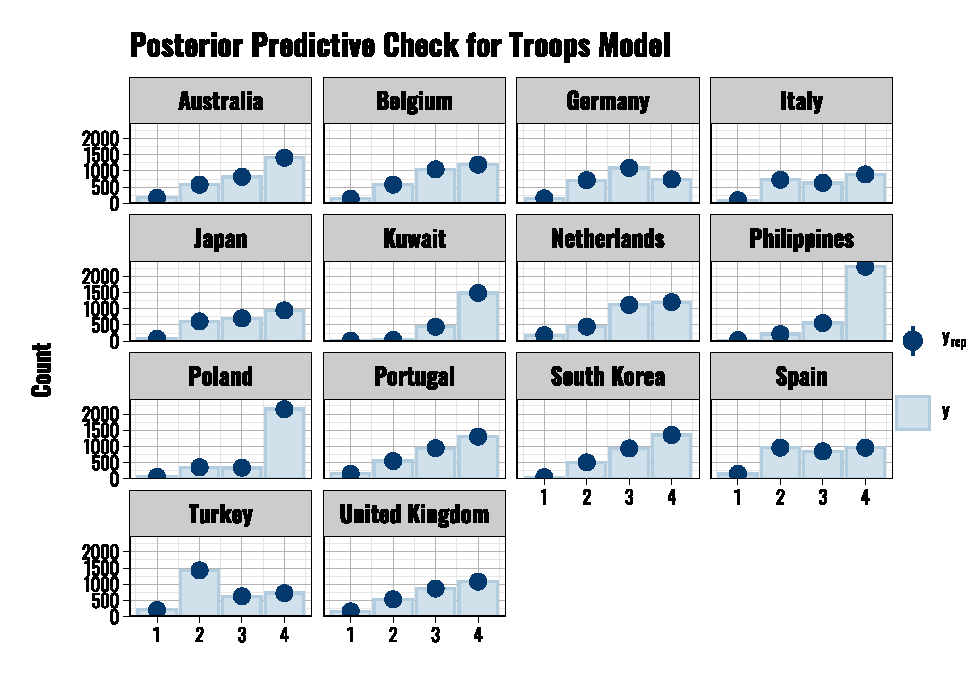
\includegraphics{02-contact-benefits_files/figure-latex/posterior-check-troops-1.pdf}
\caption{\label{fig:posterior-check-troops}Posterior predictive checks for contact models and attitudes towards the US troops outcome variable.}
\end{figure}

\begin{figure}
\centering
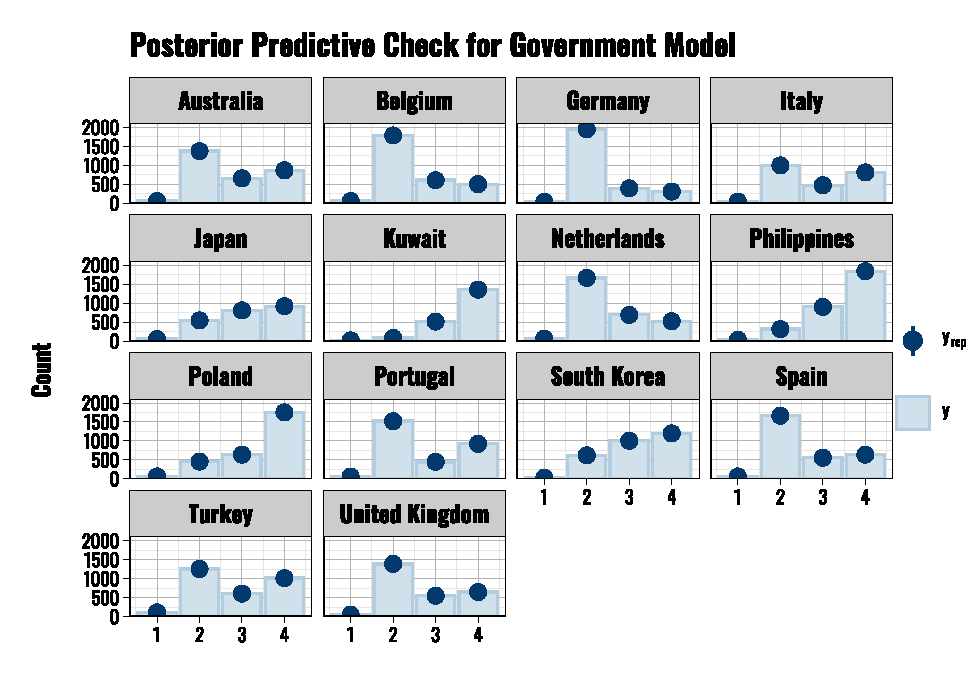
\includegraphics{02-contact-benefits_files/figure-latex/posterior-check-gov-1.pdf}
\caption{\label{fig:posterior-check-gov}Posterior predictive checks for contact models and attitudes towards the US government outcome variable.}
\end{figure}

\begin{figure}
\centering
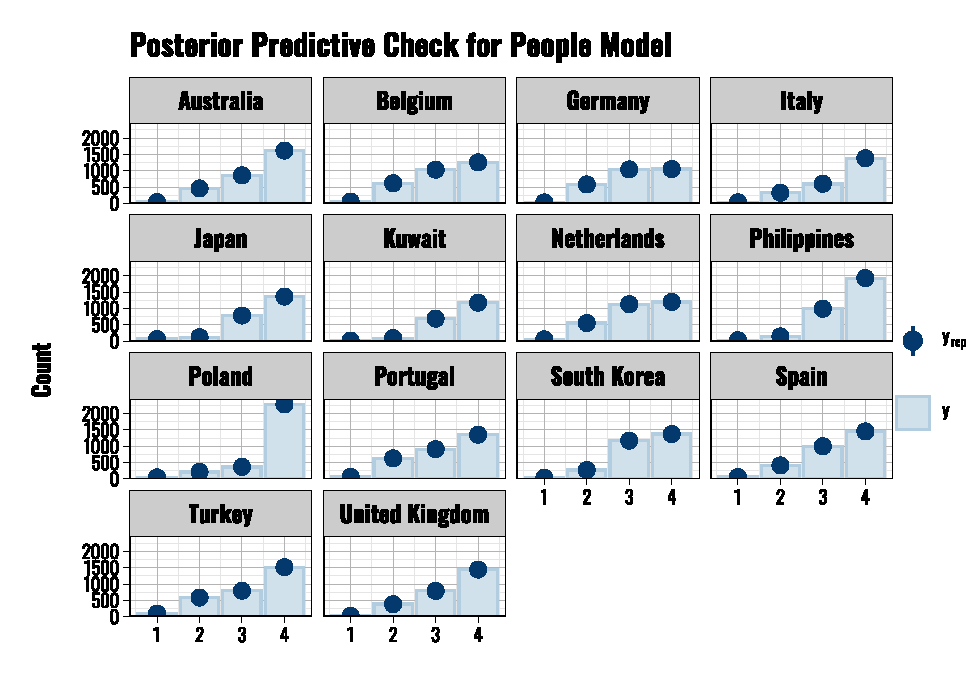
\includegraphics{02-contact-benefits_files/figure-latex/posterior-check-people-1.pdf}
\caption{\label{fig:posterior-check-people}Posterior predictive checks for contact models and attitudes towards the US people outcome variable.}
\end{figure}

\hypertarget{variables-and-model-specifications}{%
\section{Variables and Model Specifications}\label{variables-and-model-specifications}}

In the main text of the book we present the findings from a number of different models. We provide additional information here detailing the specifications of these different models, including data sources and transformations.

The opinion data we use come from a three-year long series of public opinion surveys conducted across 14 different countries. These data were collected using a research grant from the United States Department of Defense's Minerva Research Initiative. All of the individual-level variables we use in the analysis are from this original data set. With the exception of the outcome variables we use to assess attitudes towards different U.S. actors, all of the variables used in the models retain their original forms as described in the survey. The outcome variables are condensed into general categories indicating whether or not respondents express a 1) positive, 2) negative, 3) neutral, or 4) don't know/decline to answer response. We used the first year of these data in our earlier research on the subject (see \citet{Allen2020}) We provide more details in the main text.

We also use a variety of country-level variables in our models, described below.

First, we measure the respondent's country's level of democracy using data from the Varieties of Democracy Project \citep{VDemV111, Vdemcodebook2021}. Specifically, we use the \texttt{v2x\_polyarchy} variable. This variable is a composite of other indicator variables that code various aspects of a country's democratic performance. This variable runs from 0 to 1 with higher values indicating more democratic countries and lower values indicating less democratic countries.

Second, we also include variables that measure the country's total population and its gross domestic product (GDP). We obtain these data from the World Bank's World Development Indicators dataset using the \texttt{\{wbstats\}} software package for R \citep{wdidata2021, piburn2020}. Specifically, we use the SP.POP.TOTL and NY.GDP.MKTP.KD variables.

Third, we include measures of the number of U.S. military personnel deployed to the host country in a given year. To generate these values we use data obtained from the \texttt{\{troopdata\}} software package for R \citep{allenflynnmartinezmachain2022}. These data originally come from the Defense Manpower Data Center and were initially compiled by \citet{Kane2004}.

Fourth, we include a count of the number of U.S. military bases within each region of the host country. We generate these variables using data from David Vine {[}Vine2015{]} contained in the \texttt{\{troopdata\}} package. We used the \texttt{\{raster\}} software package in R \citep{hijmans2022} to generate shapefiles using the Database of Global Administrative Areas (GADM) \citep{GADM2021}. We then use the \texttt{\{sp\}} software package to check for overlap between base locations and administrative regions. We then take the sum of the base locations that fall within each administrative area.

When running our models we use a standardized version of each of these variables. Specifically, this means that each value is divided by two standard deviations. While this can offer a number of benefits in interpreting variables (see \citet{Gelman2008}) this approach also provides computational advantages by rescaling the predictor variables and reducing the variability in their range.

\hypertarget{reported-crime}{%
\chapter{Reported Crime}\label{reported-crime}}

This appendix chapter contains supplementary information corresponding to Chapter 2 on interpersonal contact and economic benefits.

\hypertarget{supplementary-figures-on-reported-crime}{%
\section{Supplementary Figures on Reported Crime}\label{supplementary-figures-on-reported-crime}}

\begin{figure}
\centering
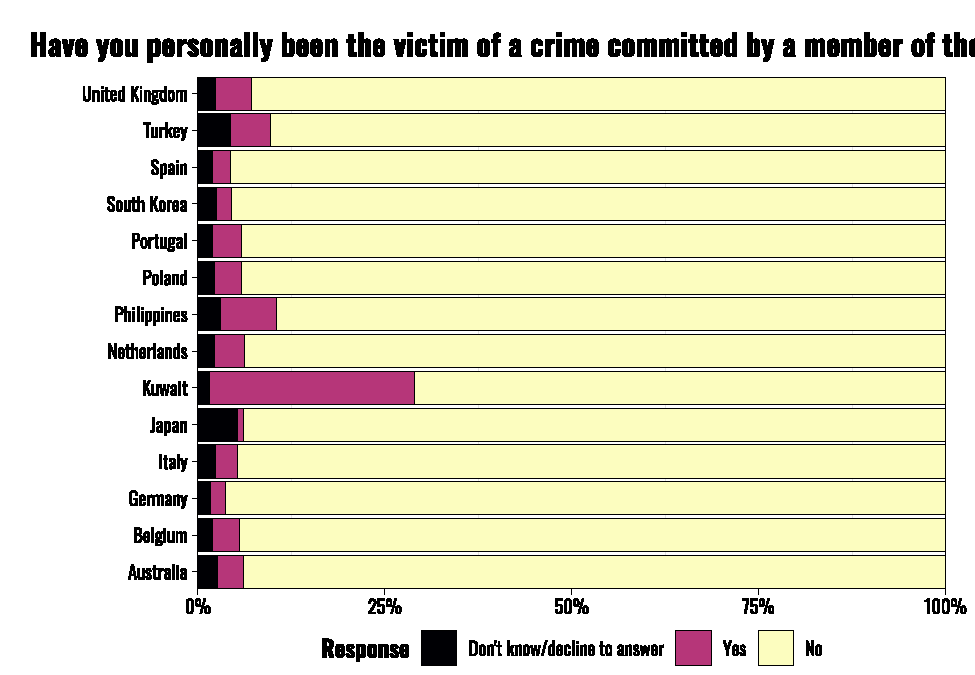
\includegraphics{03-crime_files/figure-latex/troops-crime-pers-1.pdf}
\caption{\label{fig:troops-crime-pers}Rates of reported instances of crime experienced by respondents across surveyed countries.}
\end{figure}

\begin{figure}
\centering
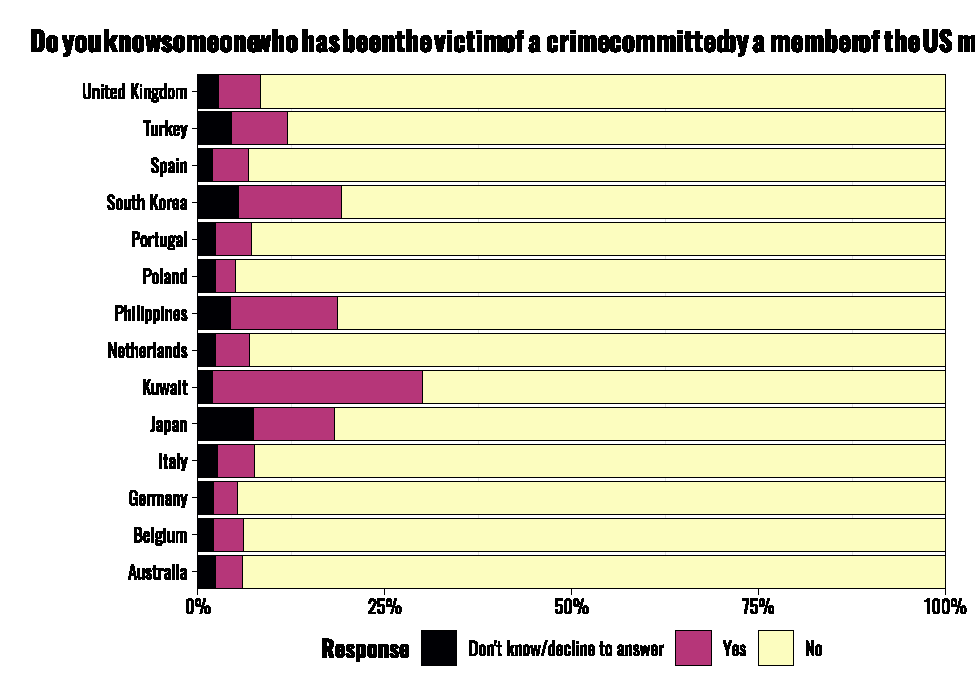
\includegraphics{03-crime_files/figure-latex/troops-crime-nonpers-1.pdf}
\caption{\label{fig:troops-crime-nonpers}Rates of reported instances of crime experienced within social networks across surveyed countries.}
\end{figure}

\hypertarget{prior-specification-tables-for-crime-models}{%
\subsection{Prior Specification Tables for Crime Models}\label{prior-specification-tables-for-crime-models}}

\begin{table}

\caption{\label{tab:prior-info-crime-troops}Priors specifications for Troops contact models.}
\centering
\fontsize{11}{13}\selectfont
\begin{tabular}[t]{l|l|l|l|l|l|l|l|l|l}
\hline
prior & class & coef & group & resp & dpar & nlpar & lb & ub & source\\
\hline
normal(0,2) & b &  &  &  & mudk &  &  &  & default\\
\hline
normal(-0.16,0.17) & b & age25to34years &  &  & mudk &  &  &  & \\
\hline
normal(-0.41,0.17) & b & age35to44years &  &  & mudk &  &  &  & \\
\hline
normal(-0.36,0.18) & b & age45to54years &  &  & mudk &  &  &  & \\
\hline
normal(-0.75,0.19) & b & age55to64years &  &  & mudk &  &  &  & \\
\hline
normal(-0.98,0.23) & b & ageAge65orolder &  &  & mudk &  &  &  & \\
\hline
normal(-0.56,0.3) & b & american\_inf\_1Alittle &  &  & mudk &  &  &  & \\
\hline
normal(-0.25,0.3) & b & american\_inf\_1Alot &  &  & mudk &  &  &  & \\
\hline
normal(0.55,0.32) & b & american\_inf\_1DontknowDdeclinetoanswer &  &  & mudk &  &  &  & \\
\hline
normal(-0.13,0.29) & b & american\_inf\_1Some &  &  & mudk &  &  &  & \\
\hline
normal(2.12,0.18) & b & american\_inf\_2DontknowDdeclinetoanswer &  &  & mudk &  &  &  & \\
\hline
normal(0.33,0.15) & b & american\_inf\_2Negative &  &  & mudk &  &  &  & \\
\hline
normal(0.24,0.18) & b & american\_inf\_2Positive &  &  & mudk &  &  &  & \\
\hline
normal(0.64,0.28) & b & american\_inf\_2Verynegative &  &  & mudk &  &  &  & \\
\hline
normal(0.48,0.41) & b & american\_inf\_2Verypositive &  &  & mudk &  &  &  & \\
\hline
 & b & basecount\_z &  &  & mudk &  &  &  & default\\
\hline
normal(0.34,0.23) & b & benefit\_nonpersDontknowDdeclinetoanswer &  &  & mudk &  &  &  & \\
\hline
normal(-0.47,0.46) & b & benefit\_nonpersYes &  &  & mudk &  &  &  & \\
\hline
normal(0.44,0.24) & b & benefit\_persDontknowDdeclinetoanswer &  &  & mudk &  &  &  & \\
\hline
normal(-0.43,0.43) & b & benefit\_persYes &  &  & mudk &  &  &  & \\
\hline
normal(-0.7,0.28) & b & contact\_nonpersDontknowDdeclinetoanswer &  &  & mudk &  &  &  & \\
\hline
normal(-0.66,0.31) & b & contact\_nonpersYes &  &  & mudk &  &  &  & \\
\hline
normal(0.56,0.29) & b & contact\_persDontknowDdeclinetoanswer &  &  & mudk &  &  &  & \\
\hline
normal(-0.71,0.37) & b & contact\_persYes &  &  & mudk &  &  &  & \\
\hline
 & b & ed\_z &  &  & mudk &  &  &  & default\\
\hline
 & b & gdp\_z &  &  & mudk &  &  &  & default\\
\hline
normal(0.08,0.11) & b & genderFemale &  &  & mudk &  &  &  & \\
\hline
normal(0.08,0.98) & b & genderNoneoftheabove &  &  & mudk &  &  &  & \\
\hline
normal(-79.98,60.28) & b & genderNonMbinary &  &  & mudk &  &  &  & \\
\hline
 & b & ideology\_z &  &  & mudk &  &  &  & default\\
\hline
 & b & income.5.cat21M40\% &  &  & mudk &  &  &  & default\\
\hline
 & b & income.5.cat41M60\% &  &  & mudk &  &  &  & default\\
\hline
 & b & income.5.cat61M80\% &  &  & mudk &  &  &  & default\\
\hline
 & b & income.5.cat81M100\% &  &  & mudk &  &  &  & default\\
\hline
 & b & minorityDeclinetoanswer &  &  & mudk &  &  &  & default\\
\hline
normal(-0.28,0.28) & b & minorityYes &  &  & mudk &  &  &  & \\
\hline
 & b & pop\_z &  &  & mudk &  &  &  & default\\
\hline
 & b & troops\_crime\_nonpersDontknowDdeclinetoanswer &  &  & mudk &  &  &  & default\\
\hline
 & b & troops\_crime\_nonpersYes &  &  & mudk &  &  &  & default\\
\hline
 & b & troops\_crime\_persDontknowDdeclinetoanswer &  &  & mudk &  &  &  & default\\
\hline
 & b & troops\_crime\_persYes &  &  & mudk &  &  &  & default\\
\hline
 & b & troops\_z &  &  & mudk &  &  &  & default\\
\hline
normal(0,2) & b &  &  &  & muneg &  &  &  & default\\
\hline
normal(0.21,0.1) & b & age25to34years &  &  & muneg &  &  &  & \\
\hline
normal(0.03,0.1) & b & age35to44years &  &  & muneg &  &  &  & \\
\hline
normal(-0.19,0.1) & b & age45to54years &  &  & muneg &  &  &  & \\
\hline
normal(-0.2,0.1) & b & age55to64years &  &  & muneg &  &  &  & \\
\hline
normal(-0.08,0.12) & b & ageAge65orolder &  &  & muneg &  &  &  & \\
\hline
normal(-0.51,0.18) & b & american\_inf\_1Alittle &  &  & muneg &  &  &  & \\
\hline
normal(-0.04,0.17) & b & american\_inf\_1Alot &  &  & muneg &  &  &  & \\
\hline
normal(-0.99,0.25) & b & american\_inf\_1DontknowDdeclinetoanswer &  &  & muneg &  &  &  & \\
\hline
normal(-0.34,0.17) & b & american\_inf\_1Some &  &  & muneg &  &  &  & \\
\hline
normal(0.42,0.17) & b & american\_inf\_2DontknowDdeclinetoanswer &  &  & muneg &  &  &  & \\
\hline
normal(1.15,0.07) & b & american\_inf\_2Negative &  &  & muneg &  &  &  & \\
\hline
normal(-0.28,0.1) & b & american\_inf\_2Positive &  &  & muneg &  &  &  & \\
\hline
normal(1.96,0.13) & b & american\_inf\_2Verynegative &  &  & muneg &  &  &  & \\
\hline
normal(-0.2,0.24) & b & american\_inf\_2Verypositive &  &  & muneg &  &  &  & \\
\hline
 & b & basecount\_z &  &  & muneg &  &  &  & default\\
\hline
normal(-0.38,0.18) & b & benefit\_nonpersDontknowDdeclinetoanswer &  &  & muneg &  &  &  & \\
\hline
normal(-0.46,0.18) & b & benefit\_nonpersYes &  &  & muneg &  &  &  & \\
\hline
normal(-0.32,0.2) & b & benefit\_persDontknowDdeclinetoanswer &  &  & muneg &  &  &  & \\
\hline
normal(-0.44,0.19) & b & benefit\_persYes &  &  & muneg &  &  &  & \\
\hline
normal(0.04,0.16) & b & contact\_nonpersDontknowDdeclinetoanswer &  &  & muneg &  &  &  & \\
\hline
normal(0.16,0.12) & b & contact\_nonpersYes &  &  & muneg &  &  &  & \\
\hline
normal(-0.1,0.22) & b & contact\_persDontknowDdeclinetoanswer &  &  & muneg &  &  &  & \\
\hline
normal(0.25,0.12) & b & contact\_persYes &  &  & muneg &  &  &  & \\
\hline
 & b & ed\_z &  &  & muneg &  &  &  & default\\
\hline
 & b & gdp\_z &  &  & muneg &  &  &  & default\\
\hline
normal(-0.1,0.06) & b & genderFemale &  &  & muneg &  &  &  & \\
\hline
normal(-0.37,0.76) & b & genderNoneoftheabove &  &  & muneg &  &  &  & \\
\hline
normal(-0.62,0.76) & b & genderNonMbinary &  &  & muneg &  &  &  & \\
\hline
 & b & ideology\_z &  &  & muneg &  &  &  & default\\
\hline
 & b & income.5.cat21M40\% &  &  & muneg &  &  &  & default\\
\hline
 & b & income.5.cat41M60\% &  &  & muneg &  &  &  & default\\
\hline
 & b & income.5.cat61M80\% &  &  & muneg &  &  &  & default\\
\hline
 & b & income.5.cat81M100\% &  &  & muneg &  &  &  & default\\
\hline
 & b & minorityDeclinetoanswer &  &  & muneg &  &  &  & default\\
\hline
normal(0.1,0.18) & b & minorityYes &  &  & muneg &  &  &  & \\
\hline
 & b & pop\_z &  &  & muneg &  &  &  & default\\
\hline
 & b & troops\_crime\_nonpersDontknowDdeclinetoanswer &  &  & muneg &  &  &  & default\\
\hline
 & b & troops\_crime\_nonpersYes &  &  & muneg &  &  &  & default\\
\hline
 & b & troops\_crime\_persDontknowDdeclinetoanswer &  &  & muneg &  &  &  & default\\
\hline
 & b & troops\_crime\_persYes &  &  & muneg &  &  &  & default\\
\hline
 & b & troops\_z &  &  & muneg &  &  &  & default\\
\hline
normal(0,2) & b &  &  &  & mupos &  &  &  & default\\
\hline
normal(-0.08,0.09) & b & age25to34years &  &  & mupos &  &  &  & \\
\hline
normal(-0.06,0.09) & b & age35to44years &  &  & mupos &  &  &  & \\
\hline
normal(-0.15,0.09) & b & age45to54years &  &  & mupos &  &  &  & \\
\hline
normal(0.06,0.09) & b & age55to64years &  &  & mupos &  &  &  & \\
\hline
normal(0.22,0.1) & b & ageAge65orolder &  &  & mupos &  &  &  & \\
\hline
normal(0.02,0.17) & b & american\_inf\_1Alittle &  &  & mupos &  &  &  & \\
\hline
normal(0.5,0.17) & b & american\_inf\_1Alot &  &  & mupos &  &  &  & \\
\hline
normal(-0.29,0.23) & b & american\_inf\_1DontknowDdeclinetoanswer &  &  & mupos &  &  &  & \\
\hline
normal(0.15,0.17) & b & american\_inf\_1Some &  &  & mupos &  &  &  & \\
\hline
normal(-0.18,0.17) & b & american\_inf\_2DontknowDdeclinetoanswer &  &  & mupos &  &  &  & \\
\hline
normal(-0.4,0.07) & b & american\_inf\_2Negative &  &  & mupos &  &  &  & \\
\hline
normal(1.17,0.06) & b & american\_inf\_2Positive &  &  & mupos &  &  &  & \\
\hline
normal(-0.61,0.17) & b & american\_inf\_2Verynegative &  &  & mupos &  &  &  & \\
\hline
normal(1.8,0.14) & b & american\_inf\_2Verypositive &  &  & mupos &  &  &  & \\
\hline
 & b & basecount\_z &  &  & mupos &  &  &  & default\\
\hline
normal(-0.2,0.15) & b & benefit\_nonpersDontknowDdeclinetoanswer &  &  & mupos &  &  &  & \\
\hline
normal(0.54,0.12) & b & benefit\_nonpersYes &  &  & mupos &  &  &  & \\
\hline
normal(-0.26,0.17) & b & benefit\_persDontknowDdeclinetoanswer &  &  & mupos &  &  &  & \\
\hline
normal(-0.09,0.13) & b & benefit\_persYes &  &  & mupos &  &  &  & \\
\hline
normal(0.13,0.13) & b & contact\_nonpersDontknowDdeclinetoanswer &  &  & mupos &  &  &  & \\
\hline
normal(0.21,0.09) & b & contact\_nonpersYes &  &  & mupos &  &  &  & \\
\hline
normal(-0.4,0.2) & b & contact\_persDontknowDdeclinetoanswer &  &  & mupos &  &  &  & \\
\hline
normal(0.58,0.1) & b & contact\_persYes &  &  & mupos &  &  &  & \\
\hline
 & b & ed\_z &  &  & mupos &  &  &  & default\\
\hline
 & b & gdp\_z &  &  & mupos &  &  &  & default\\
\hline
normal(-0.05,0.05) & b & genderFemale &  &  & mupos &  &  &  & \\
\hline
normal(-1.46,0.7) & b & genderNoneoftheabove &  &  & mupos &  &  &  & \\
\hline
normal(-0.41,0.41) & b & genderNonMbinary &  &  & mupos &  &  &  & \\
\hline
 & b & ideology\_z &  &  & mupos &  &  &  & default\\
\hline
 & b & income.5.cat21M40\% &  &  & mupos &  &  &  & default\\
\hline
 & b & income.5.cat41M60\% &  &  & mupos &  &  &  & default\\
\hline
 & b & income.5.cat61M80\% &  &  & mupos &  &  &  & default\\
\hline
 & b & income.5.cat81M100\% &  &  & mupos &  &  &  & default\\
\hline
 & b & minorityDeclinetoanswer &  &  & mupos &  &  &  & default\\
\hline
normal(0.04,0.16) & b & minorityYes &  &  & mupos &  &  &  & \\
\hline
 & b & pop\_z &  &  & mupos &  &  &  & default\\
\hline
 & b & troops\_crime\_nonpersDontknowDdeclinetoanswer &  &  & mupos &  &  &  & default\\
\hline
 & b & troops\_crime\_nonpersYes &  &  & mupos &  &  &  & default\\
\hline
 & b & troops\_crime\_persDontknowDdeclinetoanswer &  &  & mupos &  &  &  & default\\
\hline
 & b & troops\_crime\_persYes &  &  & mupos &  &  &  & default\\
\hline
 & b & troops\_z &  &  & mupos &  &  &  & default\\
\hline
normal(0,3) & Intercept &  &  &  & mudk &  &  &  & default\\
\hline
normal(0,3) & Intercept &  &  &  & muneg &  &  &  & default\\
\hline
normal(0,3) & Intercept &  &  &  & mupos &  &  &  & default\\
\hline
lkj\_corr\_cholesky(1) & L &  &  &  &  &  &  &  & default\\
\hline
 & L &  & country &  &  &  &  &  & default\\
\hline
gamma(1, 1) & sd &  &  &  & mudk &  & 0 &  & default\\
\hline
gamma(1, 1) & sd &  &  &  & muneg &  & 0 &  & default\\
\hline
gamma(1, 1) & sd &  &  &  & mupos &  & 0 &  & default\\
\hline
gamma(1, 1) & sd &  & country &  & mudk &  &  &  & default\\
\hline
 & sd & Intercept & country &  & mudk &  &  &  & default\\
\hline
gamma(1, 1) & sd &  & country &  & muneg &  &  &  & default\\
\hline
 & sd & Intercept & country &  & muneg &  &  &  & default\\
\hline
gamma(1, 1) & sd &  & country &  & mupos &  &  &  & default\\
\hline
 & sd & Intercept & country &  & mupos &  &  &  & default\\
\hline
\end{tabular}
\end{table}

\begin{table}

\caption{\label{tab:prior-info-crime-gov}Priors specifications for Government contact models.}
\centering
\fontsize{11}{13}\selectfont
\begin{tabular}[t]{l|l|l|l|l|l|l|l|l|l}
\hline
prior & class & coef & group & resp & dpar & nlpar & lb & ub & source\\
\hline
normal(0,2) & b &  &  &  & mudk &  &  &  & default\\
\hline
normal(-0.17,0.26) & b & age25to34years &  &  & mudk &  &  &  & \\
\hline
normal(0.09,0.25) & b & age35to44years &  &  & mudk &  &  &  & \\
\hline
normal(0.1,0.26) & b & age45to54years &  &  & mudk &  &  &  & \\
\hline
normal(0.05,0.27) & b & age55to64years &  &  & mudk &  &  &  & \\
\hline
normal(-0.17,0.35) & b & ageAge65orolder &  &  & mudk &  &  &  & \\
\hline
normal(-1.63,0.42) & b & american\_inf\_1Alittle &  &  & mudk &  &  &  & \\
\hline
normal(-0.98,0.38) & b & american\_inf\_1Alot &  &  & mudk &  &  &  & \\
\hline
normal(0.14,0.38) & b & american\_inf\_1DontknowDdeclinetoanswer &  &  & mudk &  &  &  & \\
\hline
normal(-0.82,0.35) & b & american\_inf\_1Some &  &  & mudk &  &  &  & \\
\hline
normal(2.05,0.25) & b & american\_inf\_2DontknowDdeclinetoanswer &  &  & mudk &  &  &  & \\
\hline
normal(0.38,0.29) & b & american\_inf\_2Negative &  &  & mudk &  &  &  & \\
\hline
normal(-0.05,0.27) & b & american\_inf\_2Positive &  &  & mudk &  &  &  & \\
\hline
normal(1.49,0.47) & b & american\_inf\_2Verynegative &  &  & mudk &  &  &  & \\
\hline
normal(1.01,0.46) & b & american\_inf\_2Verypositive &  &  & mudk &  &  &  & \\
\hline
 & b & basecount\_z &  &  & mudk &  &  &  & default\\
\hline
normal(0.07,0.3) & b & benefit\_nonpersDontknowDdeclinetoanswer &  &  & mudk &  &  &  & \\
\hline
normal(-0.57,0.49) & b & benefit\_nonpersYes &  &  & mudk &  &  &  & \\
\hline
normal(0.24,0.32) & b & benefit\_persDontknowDdeclinetoanswer &  &  & mudk &  &  &  & \\
\hline
normal(0.44,0.41) & b & benefit\_persYes &  &  & mudk &  &  &  & \\
\hline
normal(0.29,0.33) & b & contact\_nonpersDontknowDdeclinetoanswer &  &  & mudk &  &  &  & \\
\hline
normal(0.05,0.37) & b & contact\_nonpersYes &  &  & mudk &  &  &  & \\
\hline
normal(-0.28,0.39) & b & contact\_persDontknowDdeclinetoanswer &  &  & mudk &  &  &  & \\
\hline
normal(0,0.38) & b & contact\_persYes &  &  & mudk &  &  &  & \\
\hline
 & b & ed\_z &  &  & mudk &  &  &  & default\\
\hline
 & b & gdp\_z &  &  & mudk &  &  &  & default\\
\hline
normal(-0.1,0.16) & b & genderFemale &  &  & mudk &  &  &  & \\
\hline
normal(-79.93,60.03) & b & genderNoneoftheabove &  &  & mudk &  &  &  & \\
\hline
normal(1.7,0.93) & b & genderNonMbinary &  &  & mudk &  &  &  & \\
\hline
 & b & ideology\_z &  &  & mudk &  &  &  & default\\
\hline
 & b & income.5.cat21M40\% &  &  & mudk &  &  &  & default\\
\hline
 & b & income.5.cat41M60\% &  &  & mudk &  &  &  & default\\
\hline
 & b & income.5.cat61M80\% &  &  & mudk &  &  &  & default\\
\hline
 & b & income.5.cat81M100\% &  &  & mudk &  &  &  & default\\
\hline
 & b & minorityDeclinetoanswer &  &  & mudk &  &  &  & default\\
\hline
normal(-0.26,0.34) & b & minorityYes &  &  & mudk &  &  &  & \\
\hline
 & b & pop\_z &  &  & mudk &  &  &  & default\\
\hline
 & b & troops\_crime\_nonpersDontknowDdeclinetoanswer &  &  & mudk &  &  &  & default\\
\hline
 & b & troops\_crime\_nonpersYes &  &  & mudk &  &  &  & default\\
\hline
 & b & troops\_crime\_persDontknowDdeclinetoanswer &  &  & mudk &  &  &  & default\\
\hline
 & b & troops\_crime\_persYes &  &  & mudk &  &  &  & default\\
\hline
 & b & troops\_z &  &  & mudk &  &  &  & default\\
\hline
normal(0,2) & b &  &  &  & muneg &  &  &  & default\\
\hline
normal(-0.19,0.1) & b & age25to34years &  &  & muneg &  &  &  & \\
\hline
normal(-0.15,0.1) & b & age35to44years &  &  & muneg &  &  &  & \\
\hline
normal(-0.12,0.1) & b & age45to54years &  &  & muneg &  &  &  & \\
\hline
normal(0.01,0.1) & b & age55to64years &  &  & muneg &  &  &  & \\
\hline
normal(0.17,0.11) & b & ageAge65orolder &  &  & muneg &  &  &  & \\
\hline
normal(-0.12,0.17) & b & american\_inf\_1Alittle &  &  & muneg &  &  &  & \\
\hline
normal(0.08,0.17) & b & american\_inf\_1Alot &  &  & muneg &  &  &  & \\
\hline
normal(-0.72,0.22) & b & american\_inf\_1DontknowDdeclinetoanswer &  &  & muneg &  &  &  & \\
\hline
normal(-0.09,0.17) & b & american\_inf\_1Some &  &  & muneg &  &  &  & \\
\hline
normal(0.28,0.15) & b & american\_inf\_2DontknowDdeclinetoanswer &  &  & muneg &  &  &  & \\
\hline
normal(1.58,0.08) & b & american\_inf\_2Negative &  &  & muneg &  &  &  & \\
\hline
normal(-0.4,0.07) & b & american\_inf\_2Positive &  &  & muneg &  &  &  & \\
\hline
normal(2.79,0.2) & b & american\_inf\_2Verynegative &  &  & muneg &  &  &  & \\
\hline
normal(-0.61,0.21) & b & american\_inf\_2Verypositive &  &  & muneg &  &  &  & \\
\hline
 & b & basecount\_z &  &  & muneg &  &  &  & default\\
\hline
normal(-0.12,0.16) & b & benefit\_nonpersDontknowDdeclinetoanswer &  &  & muneg &  &  &  & \\
\hline
normal(-0.3,0.15) & b & benefit\_nonpersYes &  &  & muneg &  &  &  & \\
\hline
normal(-0.52,0.18) & b & benefit\_persDontknowDdeclinetoanswer &  &  & muneg &  &  &  & \\
\hline
normal(-0.21,0.16) & b & benefit\_persYes &  &  & muneg &  &  &  & \\
\hline
normal(-0.1,0.15) & b & contact\_nonpersDontknowDdeclinetoanswer &  &  & muneg &  &  &  & \\
\hline
normal(0.32,0.11) & b & contact\_nonpersYes &  &  & muneg &  &  &  & \\
\hline
normal(-0.7,0.21) & b & contact\_persDontknowDdeclinetoanswer &  &  & muneg &  &  &  & \\
\hline
normal(0.07,0.11) & b & contact\_persYes &  &  & muneg &  &  &  & \\
\hline
 & b & ed\_z &  &  & muneg &  &  &  & default\\
\hline
 & b & gdp\_z &  &  & muneg &  &  &  & default\\
\hline
normal(0.02,0.05) & b & genderFemale &  &  & muneg &  &  &  & \\
\hline
normal(-0.03,0.65) & b & genderNoneoftheabove &  &  & muneg &  &  &  & \\
\hline
normal(0.44,0.6) & b & genderNonMbinary &  &  & muneg &  &  &  & \\
\hline
 & b & ideology\_z &  &  & muneg &  &  &  & default\\
\hline
 & b & income.5.cat21M40\% &  &  & muneg &  &  &  & default\\
\hline
 & b & income.5.cat41M60\% &  &  & muneg &  &  &  & default\\
\hline
 & b & income.5.cat61M80\% &  &  & muneg &  &  &  & default\\
\hline
 & b & income.5.cat81M100\% &  &  & muneg &  &  &  & default\\
\hline
 & b & minorityDeclinetoanswer &  &  & muneg &  &  &  & default\\
\hline
normal(-0.07,0.16) & b & minorityYes &  &  & muneg &  &  &  & \\
\hline
 & b & pop\_z &  &  & muneg &  &  &  & default\\
\hline
 & b & troops\_crime\_nonpersDontknowDdeclinetoanswer &  &  & muneg &  &  &  & default\\
\hline
 & b & troops\_crime\_nonpersYes &  &  & muneg &  &  &  & default\\
\hline
 & b & troops\_crime\_persDontknowDdeclinetoanswer &  &  & muneg &  &  &  & default\\
\hline
 & b & troops\_crime\_persYes &  &  & muneg &  &  &  & default\\
\hline
 & b & troops\_z &  &  & muneg &  &  &  & default\\
\hline
normal(0,2) & b &  &  &  & mupos &  &  &  & default\\
\hline
normal(-0.06,0.1) & b & age25to34years &  &  & mupos &  &  &  & \\
\hline
normal(0.06,0.1) & b & age35to44years &  &  & mupos &  &  &  & \\
\hline
normal(-0.03,0.1) & b & age45to54years &  &  & mupos &  &  &  & \\
\hline
normal(0.04,0.1) & b & age55to64years &  &  & mupos &  &  &  & \\
\hline
normal(0.15,0.11) & b & ageAge65orolder &  &  & mupos &  &  &  & \\
\hline
normal(0.27,0.2) & b & american\_inf\_1Alittle &  &  & mupos &  &  &  & \\
\hline
normal(0.56,0.2) & b & american\_inf\_1Alot &  &  & mupos &  &  &  & \\
\hline
normal(-0.84,0.29) & b & american\_inf\_1DontknowDdeclinetoanswer &  &  & mupos &  &  &  & \\
\hline
normal(0.1,0.2) & b & american\_inf\_1Some &  &  & mupos &  &  &  & \\
\hline
normal(-0.26,0.2) & b & american\_inf\_2DontknowDdeclinetoanswer &  &  & mupos &  &  &  & \\
\hline
normal(-0.01,0.11) & b & american\_inf\_2Negative &  &  & mupos &  &  &  & \\
\hline
normal(1.39,0.07) & b & american\_inf\_2Positive &  &  & mupos &  &  &  & \\
\hline
normal(0.28,0.26) & b & american\_inf\_2Verynegative &  &  & mupos &  &  &  & \\
\hline
normal(2.28,0.14) & b & american\_inf\_2Verypositive &  &  & mupos &  &  &  & \\
\hline
 & b & basecount\_z &  &  & mupos &  &  &  & default\\
\hline
normal(-0.06,0.16) & b & benefit\_nonpersDontknowDdeclinetoanswer &  &  & mupos &  &  &  & \\
\hline
normal(0.08,0.13) & b & benefit\_nonpersYes &  &  & mupos &  &  &  & \\
\hline
normal(0.04,0.18) & b & benefit\_persDontknowDdeclinetoanswer &  &  & mupos &  &  &  & \\
\hline
normal(0.32,0.13) & b & benefit\_persYes &  &  & mupos &  &  &  & \\
\hline
normal(0.18,0.15) & b & contact\_nonpersDontknowDdeclinetoanswer &  &  & mupos &  &  &  & \\
\hline
normal(0.23,0.11) & b & contact\_nonpersYes &  &  & mupos &  &  &  & \\
\hline
normal(-0.51,0.21) & b & contact\_persDontknowDdeclinetoanswer &  &  & mupos &  &  &  & \\
\hline
normal(0.11,0.11) & b & contact\_persYes &  &  & mupos &  &  &  & \\
\hline
 & b & ed\_z &  &  & mupos &  &  &  & default\\
\hline
 & b & gdp\_z &  &  & mupos &  &  &  & default\\
\hline
normal(0.03,0.05) & b & genderFemale &  &  & mupos &  &  &  & \\
\hline
normal(-0.79,0.73) & b & genderNoneoftheabove &  &  & mupos &  &  &  & \\
\hline
normal(-0.14,0.5) & b & genderNonMbinary &  &  & mupos &  &  &  & \\
\hline
 & b & ideology\_z &  &  & mupos &  &  &  & default\\
\hline
 & b & income.5.cat21M40\% &  &  & mupos &  &  &  & default\\
\hline
 & b & income.5.cat41M60\% &  &  & mupos &  &  &  & default\\
\hline
 & b & income.5.cat61M80\% &  &  & mupos &  &  &  & default\\
\hline
 & b & income.5.cat81M100\% &  &  & mupos &  &  &  & default\\
\hline
 & b & minorityDeclinetoanswer &  &  & mupos &  &  &  & default\\
\hline
normal(0.27,0.18) & b & minorityYes &  &  & mupos &  &  &  & \\
\hline
 & b & pop\_z &  &  & mupos &  &  &  & default\\
\hline
 & b & troops\_crime\_nonpersDontknowDdeclinetoanswer &  &  & mupos &  &  &  & default\\
\hline
 & b & troops\_crime\_nonpersYes &  &  & mupos &  &  &  & default\\
\hline
 & b & troops\_crime\_persDontknowDdeclinetoanswer &  &  & mupos &  &  &  & default\\
\hline
 & b & troops\_crime\_persYes &  &  & mupos &  &  &  & default\\
\hline
 & b & troops\_z &  &  & mupos &  &  &  & default\\
\hline
normal(0,3) & Intercept &  &  &  & mudk &  &  &  & default\\
\hline
normal(0,3) & Intercept &  &  &  & muneg &  &  &  & default\\
\hline
normal(0,3) & Intercept &  &  &  & mupos &  &  &  & default\\
\hline
lkj\_corr\_cholesky(1) & L &  &  &  &  &  &  &  & default\\
\hline
 & L &  & country &  &  &  &  &  & default\\
\hline
gamma(1, 1) & sd &  &  &  & mudk &  & 0 &  & default\\
\hline
gamma(1, 1) & sd &  &  &  & muneg &  & 0 &  & default\\
\hline
gamma(1, 1) & sd &  &  &  & mupos &  & 0 &  & default\\
\hline
gamma(1, 1) & sd &  & country &  & mudk &  &  &  & default\\
\hline
 & sd & Intercept & country &  & mudk &  &  &  & default\\
\hline
gamma(1, 1) & sd &  & country &  & muneg &  &  &  & default\\
\hline
 & sd & Intercept & country &  & muneg &  &  &  & default\\
\hline
gamma(1, 1) & sd &  & country &  & mupos &  &  &  & default\\
\hline
 & sd & Intercept & country &  & mupos &  &  &  & default\\
\hline
\end{tabular}
\end{table}

\begin{table}

\caption{\label{tab:prior-info-crime-people}Priors specifications for People contact models.}
\centering
\fontsize{11}{13}\selectfont
\begin{tabular}[t]{l|l|l|l|l|l|l|l|l|l}
\hline
prior & class & coef & group & resp & dpar & nlpar & lb & ub & source\\
\hline
normal(0,2) & b &  &  &  & mudk &  &  &  & default\\
\hline
normal(0.29,0.26) & b & age25to34years &  &  & mudk &  &  &  & \\
\hline
normal(-0.01,0.28) & b & age35to44years &  &  & mudk &  &  &  & \\
\hline
normal(0.29,0.28) & b & age45to54years &  &  & mudk &  &  &  & \\
\hline
normal(0.29,0.29) & b & age55to64years &  &  & mudk &  &  &  & \\
\hline
normal(0.12,0.36) & b & ageAge65orolder &  &  & mudk &  &  &  & \\
\hline
normal(-1.06,0.43) & b & american\_inf\_1Alittle &  &  & mudk &  &  &  & \\
\hline
normal(-0.93,0.43) & b & american\_inf\_1Alot &  &  & mudk &  &  &  & \\
\hline
normal(0.1,0.43) & b & american\_inf\_1DontknowDdeclinetoanswer &  &  & mudk &  &  &  & \\
\hline
normal(-0.75,0.4) & b & american\_inf\_1Some &  &  & mudk &  &  &  & \\
\hline
normal(1.81,0.26) & b & american\_inf\_2DontknowDdeclinetoanswer &  &  & mudk &  &  &  & \\
\hline
normal(-0.39,0.3) & b & american\_inf\_2Negative &  &  & mudk &  &  &  & \\
\hline
normal(0.34,0.28) & b & american\_inf\_2Positive &  &  & mudk &  &  &  & \\
\hline
normal(0.14,0.43) & b & american\_inf\_2Verynegative &  &  & mudk &  &  &  & \\
\hline
normal(1.3,0.54) & b & american\_inf\_2Verypositive &  &  & mudk &  &  &  & \\
\hline
 & b & basecount\_z &  &  & mudk &  &  &  & default\\
\hline
normal(0.23,0.31) & b & benefit\_nonpersDontknowDdeclinetoanswer &  &  & mudk &  &  &  & \\
\hline
normal(-0.86,0.59) & b & benefit\_nonpersYes &  &  & mudk &  &  &  & \\
\hline
normal(0.1,0.34) & b & benefit\_persDontknowDdeclinetoanswer &  &  & mudk &  &  &  & \\
\hline
normal(0.81,0.41) & b & benefit\_persYes &  &  & mudk &  &  &  & \\
\hline
normal(0.43,0.33) & b & contact\_nonpersDontknowDdeclinetoanswer &  &  & mudk &  &  &  & \\
\hline
normal(-0.05,0.41) & b & contact\_nonpersYes &  &  & mudk &  &  &  & \\
\hline
normal(0.28,0.39) & b & contact\_persDontknowDdeclinetoanswer &  &  & mudk &  &  &  & \\
\hline
normal(-0.27,0.43) & b & contact\_persYes &  &  & mudk &  &  &  & \\
\hline
 & b & ed\_z &  &  & mudk &  &  &  & default\\
\hline
 & b & gdp\_z &  &  & mudk &  &  &  & default\\
\hline
normal(0.16,0.16) & b & genderFemale &  &  & mudk &  &  &  & \\
\hline
normal(1.18,1.65) & b & genderNoneoftheabove &  &  & mudk &  &  &  & \\
\hline
normal(-79.44,60.23) & b & genderNonMbinary &  &  & mudk &  &  &  & \\
\hline
 & b & ideology\_z &  &  & mudk &  &  &  & default\\
\hline
 & b & income.5.cat21M40\% &  &  & mudk &  &  &  & default\\
\hline
 & b & income.5.cat41M60\% &  &  & mudk &  &  &  & default\\
\hline
 & b & income.5.cat61M80\% &  &  & mudk &  &  &  & default\\
\hline
 & b & income.5.cat81M100\% &  &  & mudk &  &  &  & default\\
\hline
 & b & minorityDeclinetoanswer &  &  & mudk &  &  &  & default\\
\hline
normal(-0.64,0.36) & b & minorityYes &  &  & mudk &  &  &  & \\
\hline
 & b & pop\_z &  &  & mudk &  &  &  & default\\
\hline
 & b & troops\_crime\_nonpersDontknowDdeclinetoanswer &  &  & mudk &  &  &  & default\\
\hline
 & b & troops\_crime\_nonpersYes &  &  & mudk &  &  &  & default\\
\hline
 & b & troops\_crime\_persDontknowDdeclinetoanswer &  &  & mudk &  &  &  & default\\
\hline
 & b & troops\_crime\_persYes &  &  & mudk &  &  &  & default\\
\hline
 & b & troops\_z &  &  & mudk &  &  &  & default\\
\hline
normal(0,2) & b &  &  &  & muneg &  &  &  & default\\
\hline
normal(-0.12,0.1) & b & age25to34years &  &  & muneg &  &  &  & \\
\hline
normal(-0.43,0.11) & b & age35to44years &  &  & muneg &  &  &  & \\
\hline
normal(-0.36,0.11) & b & age45to54years &  &  & muneg &  &  &  & \\
\hline
normal(-0.69,0.12) & b & age55to64years &  &  & muneg &  &  &  & \\
\hline
normal(-0.41,0.13) & b & ageAge65orolder &  &  & muneg &  &  &  & \\
\hline
normal(-0.44,0.18) & b & american\_inf\_1Alittle &  &  & muneg &  &  &  & \\
\hline
normal(-0.38,0.17) & b & american\_inf\_1Alot &  &  & muneg &  &  &  & \\
\hline
normal(-0.87,0.26) & b & american\_inf\_1DontknowDdeclinetoanswer &  &  & muneg &  &  &  & \\
\hline
normal(-0.65,0.17) & b & american\_inf\_1Some &  &  & muneg &  &  &  & \\
\hline
normal(-0.14,0.2) & b & american\_inf\_2DontknowDdeclinetoanswer &  &  & muneg &  &  &  & \\
\hline
normal(1.15,0.08) & b & american\_inf\_2Negative &  &  & muneg &  &  &  & \\
\hline
normal(-0.28,0.13) & b & american\_inf\_2Positive &  &  & muneg &  &  &  & \\
\hline
normal(1.76,0.12) & b & american\_inf\_2Verynegative &  &  & muneg &  &  &  & \\
\hline
normal(0.36,0.28) & b & american\_inf\_2Verypositive &  &  & muneg &  &  &  & \\
\hline
 & b & basecount\_z &  &  & muneg &  &  &  & default\\
\hline
normal(0.26,0.19) & b & benefit\_nonpersDontknowDdeclinetoanswer &  &  & muneg &  &  &  & \\
\hline
normal(0.04,0.17) & b & benefit\_nonpersYes &  &  & muneg &  &  &  & \\
\hline
normal(-0.41,0.22) & b & benefit\_persDontknowDdeclinetoanswer &  &  & muneg &  &  &  & \\
\hline
normal(-0.13,0.19) & b & benefit\_persYes &  &  & muneg &  &  &  & \\
\hline
normal(0.07,0.17) & b & contact\_nonpersDontknowDdeclinetoanswer &  &  & muneg &  &  &  & \\
\hline
normal(0.29,0.12) & b & contact\_nonpersYes &  &  & muneg &  &  &  & \\
\hline
normal(-0.31,0.23) & b & contact\_persDontknowDdeclinetoanswer &  &  & muneg &  &  &  & \\
\hline
normal(0.04,0.13) & b & contact\_persYes &  &  & muneg &  &  &  & \\
\hline
 & b & ed\_z &  &  & muneg &  &  &  & default\\
\hline
 & b & gdp\_z &  &  & muneg &  &  &  & default\\
\hline
normal(-0.01,0.06) & b & genderFemale &  &  & muneg &  &  &  & \\
\hline
normal(0.23,1.56) & b & genderNoneoftheabove &  &  & muneg &  &  &  & \\
\hline
normal(-0.11,0.65) & b & genderNonMbinary &  &  & muneg &  &  &  & \\
\hline
 & b & ideology\_z &  &  & muneg &  &  &  & default\\
\hline
 & b & income.5.cat21M40\% &  &  & muneg &  &  &  & default\\
\hline
 & b & income.5.cat41M60\% &  &  & muneg &  &  &  & default\\
\hline
 & b & income.5.cat61M80\% &  &  & muneg &  &  &  & default\\
\hline
 & b & income.5.cat81M100\% &  &  & muneg &  &  &  & default\\
\hline
 & b & minorityDeclinetoanswer &  &  & muneg &  &  &  & default\\
\hline
normal(-0.09,0.19) & b & minorityYes &  &  & muneg &  &  &  & \\
\hline
 & b & pop\_z &  &  & muneg &  &  &  & default\\
\hline
 & b & troops\_crime\_nonpersDontknowDdeclinetoanswer &  &  & muneg &  &  &  & default\\
\hline
 & b & troops\_crime\_nonpersYes &  &  & muneg &  &  &  & default\\
\hline
 & b & troops\_crime\_persDontknowDdeclinetoanswer &  &  & muneg &  &  &  & default\\
\hline
 & b & troops\_crime\_persYes &  &  & muneg &  &  &  & default\\
\hline
 & b & troops\_z &  &  & muneg &  &  &  & default\\
\hline
normal(0,2) & b &  &  &  & mupos &  &  &  & default\\
\hline
normal(0.01,0.08) & b & age25to34years &  &  & mupos &  &  &  & \\
\hline
normal(0.08,0.08) & b & age35to44years &  &  & mupos &  &  &  & \\
\hline
normal(0.12,0.08) & b & age45to54years &  &  & mupos &  &  &  & \\
\hline
normal(0.26,0.08) & b & age55to64years &  &  & mupos &  &  &  & \\
\hline
normal(0.37,0.09) & b & ageAge65orolder &  &  & mupos &  &  &  & \\
\hline
normal(-0.27,0.16) & b & american\_inf\_1Alittle &  &  & mupos &  &  &  & \\
\hline
normal(0.38,0.16) & b & american\_inf\_1Alot &  &  & mupos &  &  &  & \\
\hline
normal(-0.7,0.2) & b & american\_inf\_1DontknowDdeclinetoanswer &  &  & mupos &  &  &  & \\
\hline
normal(-0.06,0.15) & b & american\_inf\_1Some &  &  & mupos &  &  &  & \\
\hline
normal(-0.12,0.13) & b & american\_inf\_2DontknowDdeclinetoanswer &  &  & mupos &  &  &  & \\
\hline
normal(-0.53,0.07) & b & american\_inf\_2Negative &  &  & mupos &  &  &  & \\
\hline
normal(1.25,0.06) & b & american\_inf\_2Positive &  &  & mupos &  &  &  & \\
\hline
normal(-0.96,0.12) & b & american\_inf\_2Verynegative &  &  & mupos &  &  &  & \\
\hline
normal(2.14,0.15) & b & american\_inf\_2Verypositive &  &  & mupos &  &  &  & \\
\hline
 & b & basecount\_z &  &  & mupos &  &  &  & default\\
\hline
normal(0.22,0.14) & b & benefit\_nonpersDontknowDdeclinetoanswer &  &  & mupos &  &  &  & \\
\hline
normal(0.1,0.11) & b & benefit\_nonpersYes &  &  & mupos &  &  &  & \\
\hline
normal(-0.12,0.15) & b & benefit\_persDontknowDdeclinetoanswer &  &  & mupos &  &  &  & \\
\hline
normal(0.04,0.12) & b & benefit\_persYes &  &  & mupos &  &  &  & \\
\hline
normal(-0.04,0.13) & b & contact\_nonpersDontknowDdeclinetoanswer &  &  & mupos &  &  &  & \\
\hline
normal(0.23,0.09) & b & contact\_nonpersYes &  &  & mupos &  &  &  & \\
\hline
normal(-0.48,0.18) & b & contact\_persDontknowDdeclinetoanswer &  &  & mupos &  &  &  & \\
\hline
normal(0.21,0.09) & b & contact\_persYes &  &  & mupos &  &  &  & \\
\hline
 & b & ed\_z &  &  & mupos &  &  &  & default\\
\hline
 & b & gdp\_z &  &  & mupos &  &  &  & default\\
\hline
normal(0.08,0.04) & b & genderFemale &  &  & mupos &  &  &  & \\
\hline
normal(1.76,0.88) & b & genderNoneoftheabove &  &  & mupos &  &  &  & \\
\hline
normal(-0.53,0.4) & b & genderNonMbinary &  &  & mupos &  &  &  & \\
\hline
 & b & ideology\_z &  &  & mupos &  &  &  & default\\
\hline
 & b & income.5.cat21M40\% &  &  & mupos &  &  &  & default\\
\hline
 & b & income.5.cat41M60\% &  &  & mupos &  &  &  & default\\
\hline
 & b & income.5.cat61M80\% &  &  & mupos &  &  &  & default\\
\hline
 & b & income.5.cat81M100\% &  &  & mupos &  &  &  & default\\
\hline
 & b & minorityDeclinetoanswer &  &  & mupos &  &  &  & default\\
\hline
normal(0.06,0.14) & b & minorityYes &  &  & mupos &  &  &  & \\
\hline
 & b & pop\_z &  &  & mupos &  &  &  & default\\
\hline
 & b & troops\_crime\_nonpersDontknowDdeclinetoanswer &  &  & mupos &  &  &  & default\\
\hline
 & b & troops\_crime\_nonpersYes &  &  & mupos &  &  &  & default\\
\hline
 & b & troops\_crime\_persDontknowDdeclinetoanswer &  &  & mupos &  &  &  & default\\
\hline
 & b & troops\_crime\_persYes &  &  & mupos &  &  &  & default\\
\hline
 & b & troops\_z &  &  & mupos &  &  &  & default\\
\hline
normal(0,3) & Intercept &  &  &  & mudk &  &  &  & default\\
\hline
normal(0,3) & Intercept &  &  &  & muneg &  &  &  & default\\
\hline
normal(0,3) & Intercept &  &  &  & mupos &  &  &  & default\\
\hline
lkj\_corr\_cholesky(1) & L &  &  &  &  &  &  &  & default\\
\hline
 & L &  & country &  &  &  &  &  & default\\
\hline
gamma(1, 1) & sd &  &  &  & mudk &  & 0 &  & default\\
\hline
gamma(1, 1) & sd &  &  &  & muneg &  & 0 &  & default\\
\hline
gamma(1, 1) & sd &  &  &  & mupos &  & 0 &  & default\\
\hline
gamma(1, 1) & sd &  & country &  & mudk &  &  &  & default\\
\hline
 & sd & Intercept & country &  & mudk &  &  &  & default\\
\hline
gamma(1, 1) & sd &  & country &  & muneg &  &  &  & default\\
\hline
 & sd & Intercept & country &  & muneg &  &  &  & default\\
\hline
gamma(1, 1) & sd &  & country &  & mupos &  &  &  & default\\
\hline
 & sd & Intercept & country &  & mupos &  &  &  & default\\
\hline
\end{tabular}
\end{table}

\hypertarget{posterior-predictive-check-figures-1}{%
\subsection{Posterior Predictive Check Figures}\label{posterior-predictive-check-figures-1}}

\begin{figure}
\centering
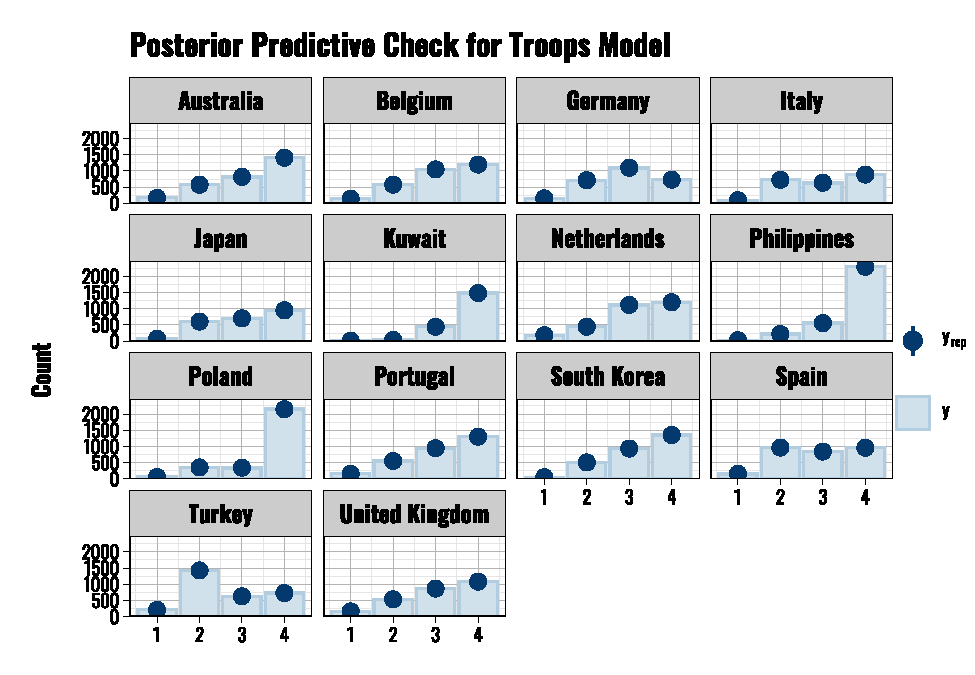
\includegraphics{03-crime_files/figure-latex/posterior-check-crime-troops-1.pdf}
\caption{\label{fig:posterior-check-crime-troops}Posterior predictive checks for contact models and attitudes towards the US troops outcome variable.}
\end{figure}

\begin{figure}
\centering
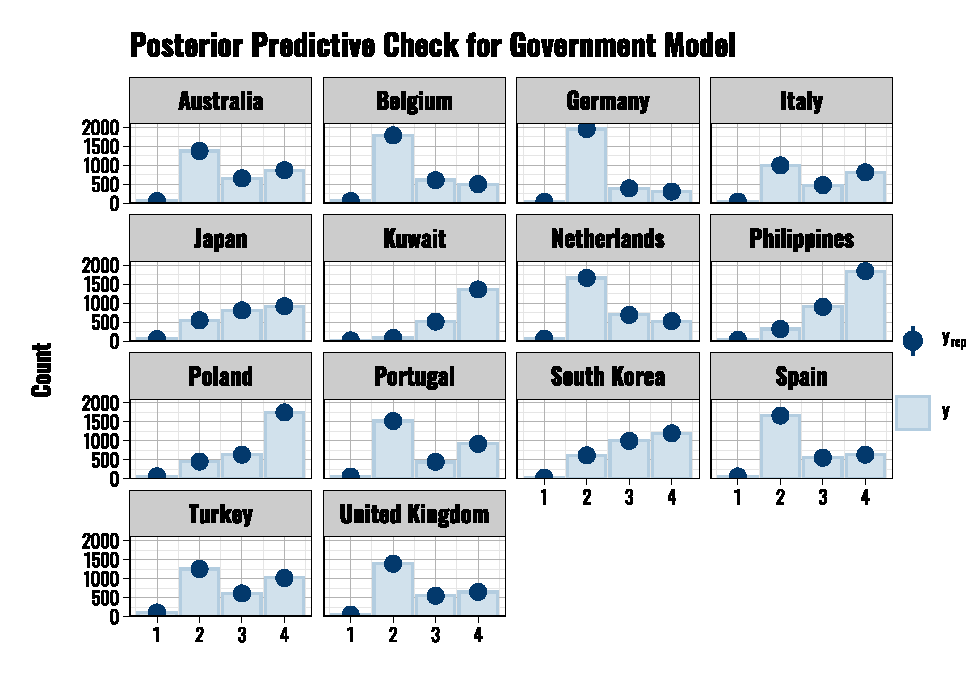
\includegraphics{03-crime_files/figure-latex/posterior-check-crime-gov-1.pdf}
\caption{\label{fig:posterior-check-crime-gov}Posterior predictive checks for contact models and attitudes towards the US government outcome variable.}
\end{figure}

\begin{figure}
\centering
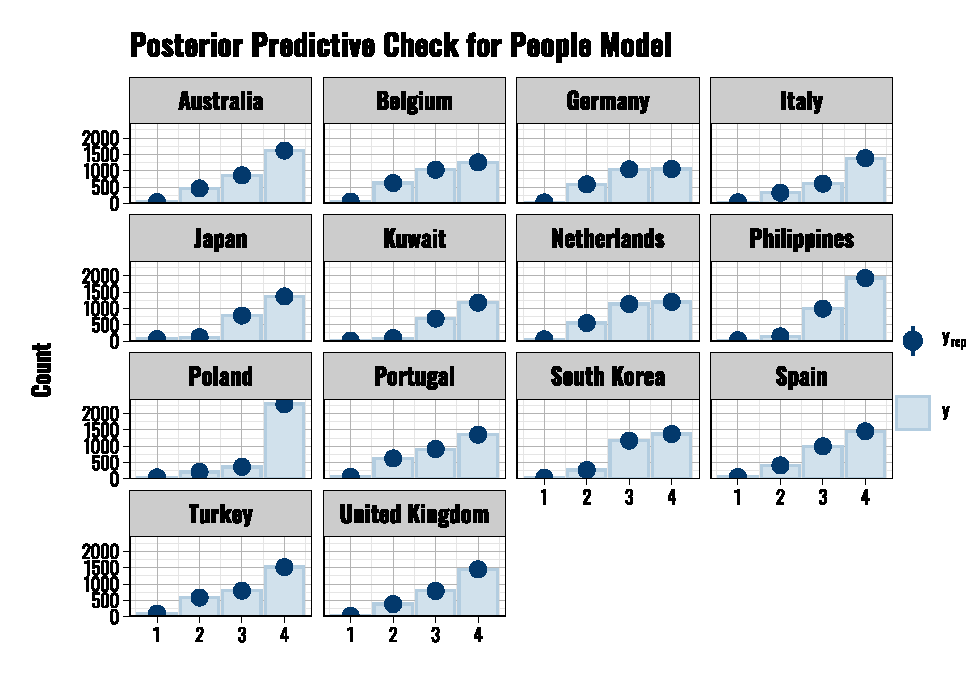
\includegraphics{03-crime_files/figure-latex/posterior-check-crime-people-1.pdf}
\caption{\label{fig:posterior-check-crime-people}Posterior predictive checks for contact models and attitudes towards the US people outcome variable.}
\end{figure}

\hypertarget{us-military-deployments-and-minority-communities}{%
\chapter{US Military Deployments and Minority Communities}\label{us-military-deployments-and-minority-communities}}

This chapter provides supplementary information related to Chapter 4 of the book, focusing on how US military deployments interact with and are viewed by minority communities.

\hypertarget{descriptive-information-1}{%
\section{Descriptive Information}\label{descriptive-information-1}}

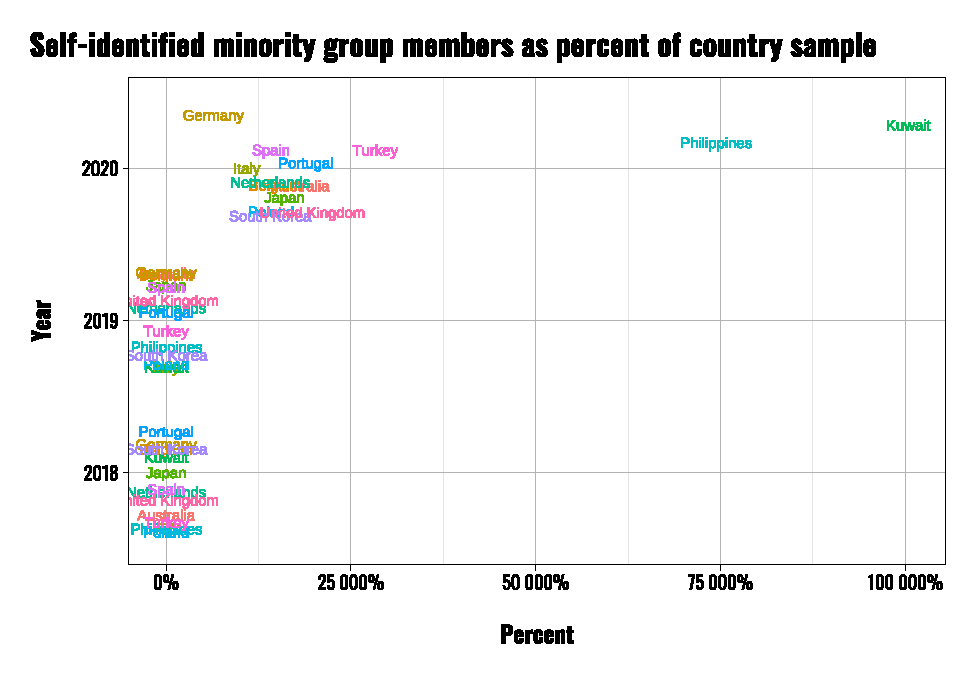
\includegraphics{04-minority_files/figure-latex/minority-description-1.pdf}

\hypertarget{blocks}{%
\chapter{Blocks}\label{blocks}}

\hypertarget{equations}{%
\section{Equations}\label{equations}}

Here is an equation.

\begin{equation} 
  f\left(k\right) = \binom{n}{k} p^k\left(1-p\right)^{n-k}
  \label{eq:binom}
\end{equation}

You may refer to using \texttt{\textbackslash{}@ref(eq:binom)}, like see Equation \eqref{eq:binom}.

\hypertarget{theorems-and-proofs}{%
\section{Theorems and proofs}\label{theorems-and-proofs}}

Labeled theorems can be referenced in text using \texttt{\textbackslash{}@ref(thm:tri)}, for example, check out this smart theorem \ref{thm:tri}.

\begin{theorem}
\protect\hypertarget{thm:tri}{}\label{thm:tri}For a right triangle, if \(c\) denotes the \emph{length} of the hypotenuse
and \(a\) and \(b\) denote the lengths of the \textbf{other} two sides, we have
\[a^2 + b^2 = c^2\]
\end{theorem}

Read more here \url{https://bookdown.org/yihui/bookdown/markdown-extensions-by-bookdown.html}.

\hypertarget{callout-blocks}{%
\section{Callout blocks}\label{callout-blocks}}

The R Markdown Cookbook provides more help on how to use custom blocks to design your own callouts: \url{https://bookdown.org/yihui/rmarkdown-cookbook/custom-blocks.html}

\hypertarget{sharing-your-book}{%
\chapter{Sharing your book}\label{sharing-your-book}}

\hypertarget{publishing}{%
\section{Publishing}\label{publishing}}

HTML books can be published online, see: \url{https://bookdown.org/yihui/bookdown/publishing.html}

\hypertarget{pages}{%
\section{404 pages}\label{pages}}

By default, users will be directed to a 404 page if they try to access a webpage that cannot be found. If you'd like to customize your 404 page instead of using the default, you may add either a \texttt{\_404.Rmd} or \texttt{\_404.md} file to your project root and use code and/or Markdown syntax.

\hypertarget{metadata-for-sharing}{%
\section{Metadata for sharing}\label{metadata-for-sharing}}

Bookdown HTML books will provide HTML metadata for social sharing on platforms like Twitter, Facebook, and LinkedIn, using information you provide in the \texttt{index.Rmd} YAML. To setup, set the \texttt{url} for your book and the path to your \texttt{cover-image} file. Your book's \texttt{title} and \texttt{description} are also used.

This \texttt{gitbook} uses the same social sharing data across all chapters in your book- all links shared will look the same.

Specify your book's source repository on GitHub using the \texttt{edit} key under the configuration options in the \texttt{\_output.yml} file, which allows users to suggest an edit by linking to a chapter's source file.

Read more about the features of this output format here:

\url{https://pkgs.rstudio.com/bookdown/reference/gitbook.html}

Or use:

\begin{Shaded}
\begin{Highlighting}[]
\NormalTok{?bookdown}\SpecialCharTok{::}\NormalTok{gitbook}
\end{Highlighting}
\end{Shaded}


  \bibliography{one.bib}

\end{document}
